\newpage
\chapter{HASIL DAN PEMBAHASAN} \label{BabIV}

% ============================================================
% 4.1 PENGUMPULAN DATA
% ============================================================
\section{Pengumpulan Data} \label{IV.PengumpulanData}
Pada tahap ini dilakukan proses pengumpulan dataset yang akan digunakan dalam penelitian ini. Dataset disusun dari dua sumber, yaitu dataset primer dan dataset sekunder. Proses pengumpulan ini bertujuan untuk menghasilkan data yang beragam dan representatif sebelum memasuki tahap anotasi dan pemodelan. Hasil pengumpulan data yang telah dilakukan disajikan dalam Tabel \ref{table:4.data_collection}.

\begin{table}[H]
    \centering
    \caption{Komposisi Dataset Awal Penelitian}
    \label{table:4.data_collection}
    \small
    \setlength{\tabcolsep}{8pt} % Menambah jarak antar kolom agar lebih renggang
    \renewcommand{\arraystretch}{1.2}
    \begin{tabular}{c l l r} % Menggunakan perataan yang lebih pas: center, left, left, right
        \hline
        \textbf{No} & \textbf{Jenis Data} & \textbf{Sumber Data} & \textbf{Jumlah} \\
        \hline
        1 & Media Sosial & Primer & 268 \\
        2 & Rekayasa \textit{Dataset} & Sekunder & 524 \\
        3 & Meme Umum (\textit{Dataset} Publik) & Sekunder & 1.500 \\
        \hline
        & \textbf{Total} & & \textbf{2.292} \\
        \hline
    \end{tabular}
\end{table}

Gambar \ref{fig:contoh_meme} di bawah ini merupakan contoh data meme yang digunakan dalam penelitian. Meme tersebut terdiri atas komponen visual berupa gambar dan komponen tekstual berupa tulisan yang saling melengkapi dalam menyampaikan makna. Kombinasi kedua komponen ini menjadi dasar dalam analisis multimodal pada penelitian ini.

\begin{figure}[H]
    \centering
    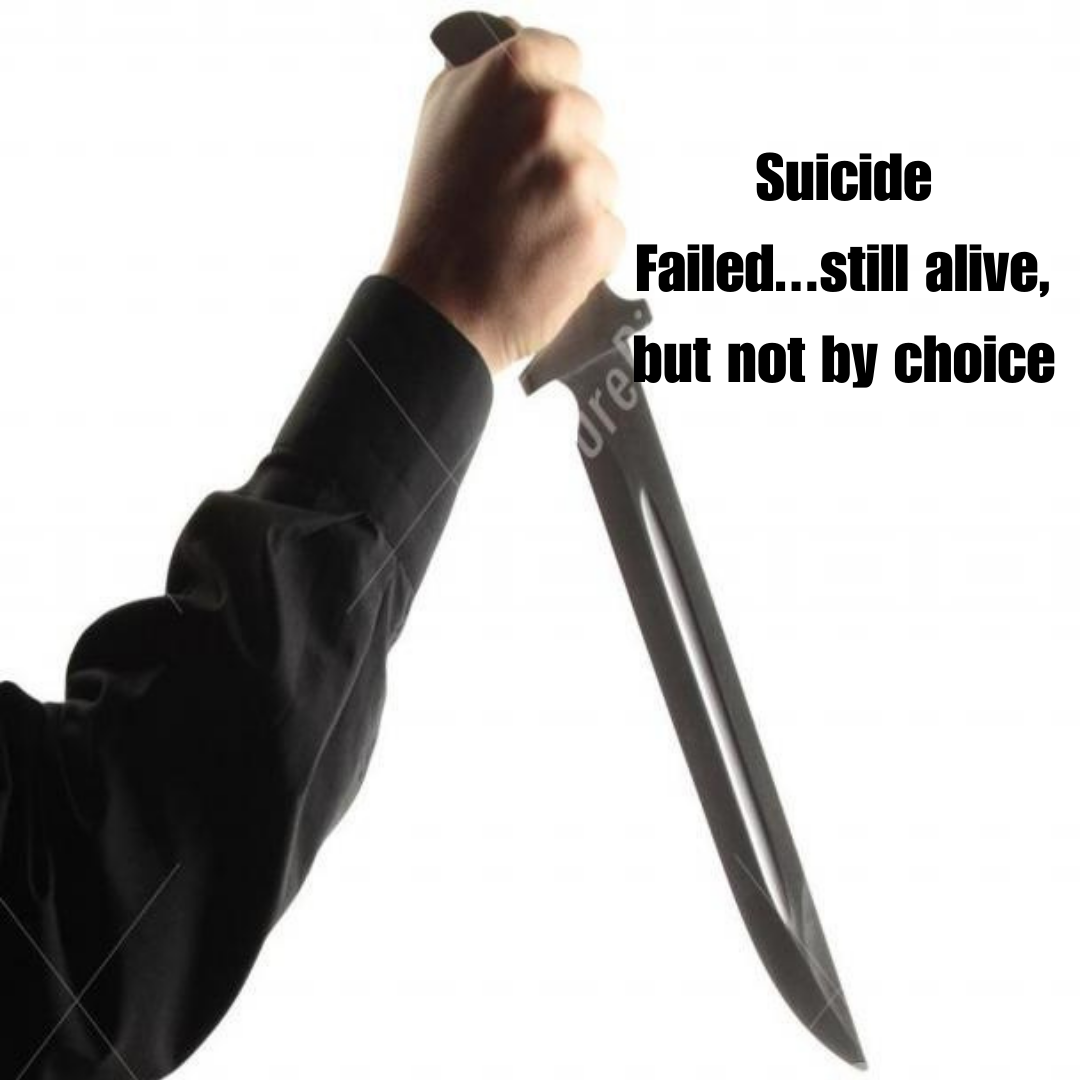
\includegraphics[width=0.4\textwidth]{figure/0085.png}
    \caption{Contoh Data Meme}
    \label{fig:contoh_meme}
\end{figure}

% ============================================================
% 4.2 HASIL ANOTASI DATA
% ============================================================
\section{Hasil Anotasi Data} \label{IV.Anotasi}

Proses anotasi data dalam penelitian ini dilakukan menggunakan pendekatan \textit{ensemble pseudo-labeling} dengan memanfaatkan dua model \textit{vision-language}, yaitu \textit{GPT-4o mini} dan \textit{Qwen-VL-Flash}, berdasarkan \textit{annotation guideline} serta kerangka \textit{RapGuard} yang telah dirancang pada Bab III. Pendekatan ini digunakan untuk menghasilkan label biner, yaitu \textit{self-harm} dan \textit{non self-harm}, dengan mempertimbangkan hubungan antara elemen visual dan tekstual pada meme.

Pada tahap awal, dataset yang dikumpulkan berjumlah 2.292. Sebelum dilakukan anotasi, dilakukan tahap \textit{pre-processing} awal berupa penyesuaian ukuran citra  agar sesuai dengan kebutuhan input model. Namun, pada tahap ini ditemukan beberapa data yang tidak dapat diproses akibat ketidaksesuaian format maupun kualitas citra yang tidak memenuhi standar. Data yang mengalami kegagalan tersebut kemudian dieliminasi dari dataset. Selain itu, dilakukan proses seleksi lebih lanjut untuk memastikan bahwa setiap data memiliki kedua modalitas, yaitu gambar dan teks. Data yang hanya terdiri dari citra tanpa teks yang dapat digunakan sebagai input multimodal juga dieliminasi, karena tidak sesuai dengan kebutuhan model yang digunakan.

Setelah seluruh proses penyaringan, diperoleh sebanyak 2.178 data yang memenuhi kriteria dan digunakan sebagai input pada proses anotasi. Setiap data kemudian diproses oleh kedua model untuk menghasilkan beberapa komponen keluaran, yaitu \textit{filename}, \textit{teks terlihat}, \textit{label}, serta relasi antara gambar dan teks. Komponen \textit{teks terlihat} digunakan sebagai representasi teks hasil ekstraksi dari meme, sedangkan \textit{label} merupakan hasil klasifikasi dalam bentuk kategori \textit{self-harm} atau \textit{non self-harm}. Adapun komponen relasi gambar dan teks digunakan sebagai informasi pendukung dalam proses peninjauan ulang secara manual, khususnya pada kasus yang mengalami perbedaan hasil anotasi (\textit{disagreement}) antar model.

Penentuan label akhir dilakukan berdasarkan konsensus antara kedua model. Pada tahap ini, komponen relasi gambar dan teks dimanfaatkan untuk membantu memahami konteks multimodal dari meme sehingga keputusan pelabelan dapat dilakukan secara lebih akurat. Selain itu, berdasarkan hasil evaluasi, komponen \textit{teks terlihat} yang dihasilkan oleh \textit{GPT-4o mini} menunjukkan tingkat kesesuaian yang lebih tinggi dibandingkan \textit{Qwen-VL-Flash}, sehingga digunakan sebagai representasi teks pada dataset akhir. Berikut adalah hasil anotasi yang dihasilkan oleh GPT-4o mini dan Qwen-VL-Flash pada beberapa data sampel.

\newcommand{\annotimg}[1]{\vspace{0pt}{\centering\includegraphics[width=0.95\linewidth,height=4cm,keepaspectratio]{#1}\par}}
\newcommand{\annottop}[1]{\vspace{0pt}{\raggedright #1\par}}
\newcommand{\annottopcenter}[1]{\vspace{0pt}{\centering #1\par}}

\begin{landscape}
\setlength{\tabcolsep}{3pt}
\renewcommand{\arraystretch}{1.1}
\begin{longtable}{|>{\centering\arraybackslash}p{4.1cm}|p{3.0cm}|>{\centering\arraybackslash}p{2cm}|p{5.8cm}|}
    \caption{Contoh Hasil Anotasi oleh GPT-4o}
    \label{table:4.contoh_anotasi_gpt4o}\\
    \hline
    \textbf{Gambar} & \textbf{Teks Terlihat} & \textbf{Label} & \textbf{Relasi Gambar dan Teks} \\
    \hline
    \endfirsthead
    \hline
    \textbf{Gambar} & \textbf{Teks Terlihat} & \textbf{Label} & \textbf{Relasi Gambar dan Teks} \\
    \hline
    \endhead
    \annotimg{figure/0771.png} & \annottop{KILL ME PLS} & \annottopcenter{SELF-HARM} & \annottop{Teks yang meminta untuk dibunuh mengubah makna gambar yang tampak netral menjadi berbahaya.} \\
    \hline
    \annotimg{figure/2093.jpg} & \annottop{"When u texted ur man 3 min ago and he still hasn't responded I'm single right now."} & \annottopcenter{NON-SELF-HARM} & \annottop{Teks menggambarkan frustrasi dalam hubungan tanpa indikasi self-harm, meskipun ada nada humor.} \\
    \hline
\end{longtable}
\end{landscape}

\begin{landscape}
\setlength{\tabcolsep}{3pt}
\renewcommand{\arraystretch}{1.1}
\begin{longtable}{|>{\centering\arraybackslash}p{4.1cm}|p{3.0cm}|>{\centering\arraybackslash}p{2cm}|p{5.8cm}|}
    \hline
    \textbf{Gambar} & \textbf{Teks Terlihat} & \textbf{Label} & \textbf{Relasi Gambar dan Teks} \\
    \hline
    \endfirsthead
    \hline
    \textbf{Gambar} & \textbf{Teks Terlihat} & \textbf{Label} & \textbf{Relasi Gambar dan Teks} \\
    \hline
    \endhead
    \annotimg{figure/0769.png} & \annottop{I WILL FIND YOU AND I WILL KILL YOU} & \annottopcenter{NON-SELF-HARM} & \annottop{Teks yang mengancam berinteraksi dengan ekspresi serius dalam gambar, tetapi tidak menunjukkan indikasi self-harm atau ideasi bunuh diri.} \\
    \hline
    \annotimg{figure/0016.png} & \annottop{The things that make me want to kill myself are permanent, so how can I ever want to live?} & \annottopcenter{SELF-HARM} & \annottop{Teks yang menyatakan keinginan untuk bunuh diri berinteraksi dengan gambar senjata, menciptakan makna yang berbahaya.} \\
    \hline
\end{longtable}
\end{landscape}

% longtable lanjutan di atas merupakan bagian dari tabel yang sama,
% sehingga counter tabel dikembalikan agar penomoran tidak melompat.
\addtocounter{table}{-1}

\begin{landscape}
\setlength{\tabcolsep}{3pt}
\renewcommand{\arraystretch}{1.1}
\begin{longtable}{|>{\centering\arraybackslash}p{3.1cm}|p{2.0cm}|>{\centering\arraybackslash}p{2cm}|p{8.2cm}|}
    \caption{Contoh Hasil Anotasi oleh Qwen-VL-Flash}
    \label{table:4.contoh_anotasi_qwenvlflash}\\
    \hline
    \textbf{Gambar} & \textbf{Teks Terlihat} & \textbf{Label} & \textbf{Relasi Gambar dan Teks} \\
    \hline
    \endfirsthead
    \hline
    \textbf{Gambar} & \textbf{Teks Terlihat} & \textbf{Label} & \textbf{Relasi Gambar dan Teks} \\
    \hline
    \endhead
    \annotimg{figure/0771.png} & \annottop{KILL ME PLS risuvach.ru} & \annottopcenter{SELF-HARM} & \annottop{Gambar wajah yang tampak buram dan menyeramkan secara visual memperkuat makna teks 'KILL ME PLS' yang secara eksplisit menyiratkan ide bunuh diri, sehingga keduanya bersatu membentuk pesan bahaya yang jelas tanpa perlu penjelasan tambahan.} \\
    \hline
    \annotimg{figure/2093.jpg} & \annottop{When u texted ur man 3 min ago and he still hasn't responded @daddyissues. I'm single right now.} & \annottopcenter{NON-SELF-HARM} & \annottop{Gambar menampilkan Rihanna dengan ekspresi tenang dan pose santai, yang kontras dengan teks yang menggambarkan kekecewaan dalam hubungan; namun tidak ada indikator visual atau teks yang menyiratkan self-harm atau ide bunuh diri, hanya humor tentang situasi cinta yang tidak seimbang.} \\
    \hline
    \annotimg{figure/0769.png} & \annottop{I WILL FIND YOU AND I WILL KILL YOU} & \annottopcenter{SELF-HARM} & \annottop{Gambar menampilkan wajah pria yang tampak serius dan mengancam sambil berbicara di telepon, yang bersama teks 'I WILL FIND YOU AND I WILL KILL YOU' menciptakan nuansa ancaman kekerasan yang dapat dikaitkan dengan ide bunuh diri atau agresi terhadap diri sendiri dalam konteks narasi kriminal atau psikologis ekstrem.} \\
    \hline
    \annotimg{figure/0016.png} & \annottop{The things that make me want to kill myself are permanent, so how can I ever want to live?} & \annottopcenter{SELF-HARM} & \annottop{Gambar emoji dengan mata 'X' dan mulut terbuka (menunjukkan keterkejutan/keputusasaan) serta revolver yang mengarah ke kepala secara visual memperkuat teks yang menyatakan keinginan bunuh diri, menciptakan interaksi yang berbahaya dan langsung mengindikasikan ide bunuh diri.} \\
    \hline
\end{longtable}
\end{landscape}

\subsection{Tingkat Kesepakatan Antar Model} \label{IV.Anotasi.Agreement}
Analisis tingkat kesepakatan (\textit{agreement}) antara \textit{GPT-4o mini} dan \textit{Qwen-VL-Flash} dilakukan untuk mengevaluasi konsistensi hasil anotasi yang dihasilkan oleh kedua model. Melalui analisis ini, dapat diketahui sejauh mana kedua model memberikan label yang sama terhadap data yang dianotasi. Tingkat kesepakatan ini menjadi indikator penting dalam menilai reliabilitas pendekatan \textit{ensemble pseudo-labeling} yang digunakan dalam penelitian ini.

Hasil analisis menunjukkan bahwa sebagian besar data memiliki label yang konsisten antara kedua model, yang mengindikasikan bahwa pendekatan \textit{ensemble pseudo-labeling} yang digunakan memiliki tingkat reliabilitas yang baik. Namun, pada sebagian data lainnya ditemukan perbedaan hasil anotasi (\textit{disagreement}). Data dengan hasil \textit{disagreement} kemudian ditinjau ulang secara manual oleh peneliti untuk menentukan label akhir. Proses peninjauan ini dilakukan dengan mengacu pada \textit{annotation guideline} yang telah disusun, serta mempertimbangkan hasil ekstraksi teks (\textit{Optical Character Recognition}/OCR) yang dihasilkan oleh model, khususnya dari \textit{GPT-4o}, guna memastikan interpretasi teks pada meme dilakukan secara akurat. Distribusi tingkat kesepakatan antar model disajikan pada Tabel \ref{table:4.agreement_distribution} di bawah ini.

\begin{table}[H]
    \centering
    \caption{Distribusi Tingkat Kesepakatan Antar Model}
    \label{table:4.agreement_distribution}
    \small
    \setlength{\tabcolsep}{3pt}
    \renewcommand{\arraystretch}{1.1}
    \begin{tabular}{p{2.5cm} p{2.5cm} p{2cm}}
        \hline
        \textbf{Kategori} & \textbf{Jumlah Data} & \textbf{Persentase} \\
        \hline
        \textit{Agreement} & 2.068 & 94,95\% \\
        \textit{Disagreement} & 110 & 5,05\% \\
        \textbf{Total} & \textbf{2.178} & \textbf{100\%} \\
        \hline
    \end{tabular}
\end{table}

\subsection{Distribusi Label Akhir} \label{IV.Anotasi.Distribusi}

Setelah proses anotasi dan penentuan label akhir melalui pengecekan manual oleh peneliti, diperoleh distribusi data berdasarkan kategori \textit{self-harm} dan \textit{non self-harm}. Distribusi ini penting untuk memahami keseimbangan data yang akan digunakan pada tahap pelatihan model. Distribusi label akhir disajikan pada Tabel \ref{table:4.distribusi_label} di bawah ini.

\begin{table}[H]
    \centering
    \caption{Distribusi Label Akhir Dataset}
    \label{table:4.distribusi_label}
    \small
    \setlength{\tabcolsep}{3pt}
    \renewcommand{\arraystretch}{1.1}
    \begin{tabular}{p{2.5cm} p{2.5cm} p{2cm}}
        \hline
        \textbf{Label} & \textbf{Jumlah Data} & \textbf{Persentase} \\
        \hline
        \textit{Self-harm} & 653 & 30\% \\
        \textit{Non self-harm} & 1.525 & 70\% \\
        \textbf{Total} & \textbf{2.178} & \textbf{100\%} \\
        \hline
    \end{tabular}
\end{table}

Berdasarkan hasil tersebut, terlihat bahwa distribusi data tidak seimbang (\textit{imbalanced}), di mana jumlah data pada kelas \textit{non self-harm} lebih banyak dibandingkan dengan kelas \textit{self-harm}. Kondisi ini merupakan hal yang umum dalam studi terkait deteksi \textit{self-harm}, terutama pada data yang bersumber dari internet, sehingga tidak dilakukan \textit{pre-processing} seperti \textit{oversampling} atau \textit{undersampling} dalam penelitian ini. Hal ini disebabkan karena konten \textit{self-harm} memiliki prevalensi yang relatif lebih rendah, sering kali tersirat, dan tidak selalu terlaporkan secara eksplisit dalam data dunia nyata. Distribusi data yang tidak seimbang pada penelitian ini tetap dipertahankan agar sesuai dengan karakteristik alami data \textit{self-harm} di dunia nyata, sehingga hasil yang diperoleh dapat merepresentasikan kondisi sebenarnya di lapangan.

% ============================================================
% 4.3 HASIL PRE-PROCESSING DATA
% ============================================================
\section{Hasil \textit{Pre-processing} Data} \label{IV.Preprocessing}
Pada penelitian ini, tahap \textit{pre-processing} tidak dilakukan sepenuhnya secara manual, melainkan terintegrasi langsung ke dalam \textit{pipeline} pelatihan model multimodal. Data teks dibaca dari kolom \textit{Teks Terlihat}, sedangkan data gambar diambil dari direktori dataset yang telah ditetapkan. Pendekatan ini dipilih karena sebagian besar proses penyesuaian input telah ditangani oleh komponen bawaan model, yaitu \textit{tokenizer ELECTRA} untuk modalitas teks dan \textit{CLIPImageProcessor} untuk modalitas gambar. Dengan demikian, data dapat diproses secara lebih efisien dan konsisten sesuai kebutuhan arsitektur model.

Secara umum, tahap \textit{pre-processing} dalam penelitian ini meliputi tiga bagian utama, yaitu \textit{pre-processing} modalitas gambar, \textit{pre-processing} modalitas teks, dan pembagian dataset. Pada modalitas gambar, proses utama meliputi pembacaan citra, konversi ke format RGB, augmentasi pada data latih, serta pemrosesan otomatis menggunakan \textit{processor CLIP}. Pada modalitas teks, proses utama dilakukan melalui tokenisasi otomatis menggunakan \textit{tokenizer ELECTRA} tanpa tahapan pembersihan teks secara manual. Setelah kedua modalitas siap digunakan, dataset kemudian dibagi menjadi data pelatihan dan data validasi menggunakan pendekatan \textit{stratified split} agar distribusi kelas tetap terjaga.

\subsection{\textit{Pre-processing} Gambar} \label{IV.Preprocessing.Gambar}
Gambar pada penelitian ini dilakukan melalui dua tahap utama, yaitu augmentasi data pada data pelatihan dan pemrosesan otomatis menggunakan \textit{processor} CLIP.  Pada modalitas gambar dikonversi ke format RGB agar memiliki representasi warna yang seragam. Setelah itu, pada data latih diterapkan augmentasi untuk meningkatkan variasi data dan membantu model menjadi lebih \textit{robust} terhadap perubahan visual yang masih wajar. Data validasi tidak diberikan augmentasi agar proses evaluasi tetap merepresentasikan kondisi data asli.

Augmentasi yang digunakan pada implementasi ini terdiri atas tiga transformasi utama. Pertama, \textit{RandomHorizontalFlip()} untuk membalik gambar secara horizontal secara acak. Kedua, \textit{RandomRotation(degrees=15)} untuk memberikan rotasi acak hingga 15 derajat. Ketiga, \textit{ColorJitter(brightness=0.2, contrast=0.2, saturation=0.2, hue=0.1)} untuk menghasilkan variasi pada aspek kecerahan, kontras, saturasi, dan \textit{hue}. Kombinasi ketiga augmentasi tersebut bertujuan untuk memperkaya distribusi visual data tanpa mengubah makna utama gambar secara berlebihan.

Setelah tahap augmentasi, gambar diproses menggunakan \textit{CLIPImageProcessor} dari model \textit{openai/clip-vit-base-patch32}. Pada tahap ini, gambar diubah menjadi \textit{pixel\_values} yang siap digunakan sebagai input bagi \textit{encoder} visual CLIP. Proses seperti normalisasi nilai piksel, penyesuaian ukuran input, dan perubahan format tensor tidak dilakukan secara manual oleh peneliti, melainkan dilakukan secara otomatis oleh \textit{processor} CLIP sebagai bagian dari \textit{pipeline} model. Pendekatan ini membuat proses \textit{pre-processing} gambar menjadi lebih praktis dan tetap konsisten dengan kebutuhan model \textit{pra-latih} yang digunakan.
Berikut potongan kode implementasi \textit{pre-processing} gambar yang dilakukan pada penelitian ini.

\begin{lstlisting}[caption={Kode \textit{Pre-processing} Gambar}, label={code:4.preprocessing_gambar}]
if self.is_train:
    self.augmentation = transforms.Compose([
        transforms.RandomHorizontalFlip(),
        transforms.RandomRotation(degrees=15),
        transforms.ColorJitter(
            brightness=0.2,
            contrast=0.2,
            saturation=0.2,
            hue=0.1
        ),
    ])
else:
    self.augmentation = None

image = Image.open(img_path).convert('RGB')

image_for_clip = image
if self.is_train and self.augmentation:
    image_for_clip = self.augmentation(image)

clip_inputs = self.clip_processor(images=image_for_clip, return_tensors='pt')
pixel_values = clip_inputs['pixel_values'].squeeze(0)
\end{lstlisting}


\subsection{\textit{Pre-processing} Teks} \label{IV.Preprocessing.Teks}

Pada modalitas teks, data diambil dari kolom \textit{Teks Terlihat} pada file CSV hasil anotasi GPT-4o. Dalam implementasi penelitian ini, tidak dilakukan tahap pembersihan teks secara manual seperti \textit{case folding}, \textit{stopword removal}, \textit{stemming}, maupun \textit{lemmatization}. Sebaliknya, proses \textit{pre-processing} dilakukan langsung oleh \textit{tokenizer} bawaan model ELECTRA yang dipanggil melalui \textit{AutoTokenizer}. Pendekatan ini dipilih agar pemrosesan teks tetap konsisten dengan kebutuhan model \textit{transformer} yang digunakan.

Tokenizer yang digunakan dimuat dari model \textit{sentinet/suicidality}, yang pada \textit{pipeline} ini berfungsi sebagai \textit{tokenizer} untuk \textit{encoder} teks ELECTRA. Setiap teks diproses dengan beberapa parameter penting, yaitu \textit{truncation=True} untuk memotong teks yang melebihi panjang maksimum, \textit{padding='max\_length'} untuk menyamakan panjang seluruh input, \textit{max\_length=128} untuk menetapkan batas maksimum token, dan \textit{return\_tensors='pt'} agar hasil tokenisasi langsung berbentuk tensor PyTorch. Dari proses ini dihasilkan dua komponen utama, yaitu \textit{input\_ids} dan \textit{attention\_mask}. \textit{input\_ids} merupakan representasi numerik dari token hasil tokenisasi, sedangkan \textit{attention\_mask} berfungsi menandai token yang valid dan token hasil \textit{padding}. Berikut potongan kode implementasi \textit{pre-processing} teks yang dilakukan pada penelitian ini.

\begin{lstlisting}[caption={Kode \textit{Pre-processing} Teks}, label={code:4.preprocessing_teks}]
text = str(row['Teks Terlihat']) if 'Teks Terlihat' in row else ''

enc = self.electra_tokenizer(
    text,
    truncation=True,
    padding='max_length',
    max_length=self.max_len,
    return_tensors='pt'
)

input_ids = enc['input_ids'].squeeze(0)
attention_mask = enc['attention_mask'].squeeze(0)
\end{lstlisting}

Berdasarkan implementasi tersebut, \textit{pre-processing} teks pada penelitian ini ditangani oleh \textit{tokenizer} model. Pendekatan ini menjadikan proses pemrosesan teks lebih efisien, terstandarisasi, dan sesuai dengan format input yang dibutuhkan oleh ELECTRA sebagai \textit{text encoder}.

\subsection{Pembagian Dataset} \label{IV.Preprocessing.Split}
Pembagian dataset dilakukan secara acak (\textit{random splitting}) menggunakan fungsi \textit{train\_test\_split()} dari  \textit{library scikit-learn} dengan rasio 80:20 antara data latih (\textit{training set}) dan data validasi (\textit{validation set}). Parameter \textit{random\_state=42} digunakan untuk memastikan bahwa proses pembagian data bersifat konsisten dan dapat direproduksi pada setiap eksperimen. Selain itu, parameter \textit{stratify=labels\_df['Label']} diterapkan untuk menjaga proporsi distribusi kelas pada data latih dan data validasi tetap serupa dengan distribusi data awal. Berikut kode implementasi pembagian dataset yang digunakan.

\begin{lstlisting}[caption={Kode Pembagian Dataset}, label={code:4.pembagian_dataset}]
labels_df = pd.read_csv(config.LABELS_CSV)
label_mapping = {'NON-SELF-HARM': 0, 'SELF-HARM': 1}

labels_df = labels_df[labels_df['Label Akhir'].isin(label_mapping.keys())].copy()
labels_df['Label'] = labels_df['Label Akhir'].map(label_mapping)

train_df, val_df = train_test_split(
    labels_df,
    test_size=0.2,
    random_state=config.SEED,
    stratify=labels_df['Label']
)
\end{lstlisting}

Berdasarkan implementasi tersebut, dataset dibagi menjadi dua subset, yaitu data latih dan data validasi, tanpa adanya pemisahan \textit{test set} secara terpisah. Oleh karena itu, proses evaluasi model selama eksperimen dilakukan menggunakan data validasi. Pendekatan ini memungkinkan penilaian performa model secara langsung selama proses pengembangan, meskipun belum mencakup evaluasi akhir menggunakan data uji yang benar-benar independen. Berikut adalah hasil pembagian dataset yang diperoleh setelah proses \textit{train\_test\_split} dilakukan, yang disajikan dalam Tabel \ref{table:4.datasplit} di bawah ini.

\begin{table}[H]
    \centering
    \caption{Pembagian Dataset}
    \label{table:4.datasplit}
    \small
    \setlength{\tabcolsep}{3pt}
    \renewcommand{\arraystretch}{1.1}
    \begin{tabular}{p{2.1cm} p{2cm} p{2cm} p{1.2cm}}
        \hline
        \textbf{Split} & \textbf{\textit{Self-Harm}} & \textbf{\textit{Non-Self-Harm}} & \textbf{Total} \\
        \hline
        \textit{Training} & 522 & 1.220 & 1.742 \\
        \textit{Validation} & 131 & 305 & 436 \\
        \textbf{Total} & \textbf{653} & \textbf{1.525} & \textbf{2.178} \\
        \hline
    \end{tabular}
\end{table}

% ============================================================
% 4.4 HASIL PENGEMBANGAN MODEL
% ============================================================
\section{Hasil Pengembangan Model Multimodal} \label{IV.Model}
Pada tahap pengembangan model, arsitektur yang telah dirancang pada Bab III direalisasikan ke dalam bentuk implementasi yang digunakan pada proses eksperimen. Fokus pada subbab ini bukan lagi menjelaskan teori atau rancangan konseptual model, melainkan menjabarkan konfigurasi model yang benar-benar diterapkan, termasuk komponen yang dibekukan (\textit{freeze}), komponen yang dilatih (\textit{trainable}), serta alur representasi fitur dari masing-masing modalitas hingga menghasilkan prediksi kelas.

\subsection{Konfigurasi Model} \label{IV.Model.Konfigurasi}
Berdasarkan implementasi yang telah dilakukan penelitian ini, terdapat tiga kelompok model utama, yaitu model unimodal gambar, model unimodal teks, dan model multimodal. Model unimodal digunakan sebagai \textit{baseline} untuk mengevaluasi kemampuan masing-masing modalitas secara independen, sedangkan model multimodal digunakan untuk menganalisis pengaruh penggabungan informasi visual dan tekstual dalam tugas klasifikasi meme \textit{self-harm}.


\subsubsection{Model unimodal Gambar}
\label{IV.Model.Konfigurasi.UnimodalGambar}

Model unimodal gambar diimplementasikan sebagai \textit{baseline} untuk mengevaluasi kemampuan representasi visual secara independen. Pada konfigurasi ini, hanya fitur visual dari CLIP yang digunakan, sedangkan modalitas teks dinonaktifkan. Fitur gambar diproses oleh \textit{image encoder} CLIP untuk menghasilkan \textit{embedding} visual berdimensi 512. \textit{Embedding} tersebut kemudian dinormalisasi menggunakan \textit{L2 normalization} agar berada pada ruang fitur yang stabil. Selanjutnya, fitur hasil normalisasi diteruskan ke \textit{classifier} berbasis MLP untuk menghasilkan prediksi kelas.

Untuk menjaga konsistensi dengan arsitektur multimodal, representasi teks tetap disertakan dalam bentuk vektor nol (\textit{zero vector}) berdimensi 256, kemudian dikonkatenasikan dengan fitur gambar sehingga menghasilkan representasi gabungan berdimensi 768. Namun, informasi efektif tetap hanya berasal dari modalitas gambar. Potongan kode implementasinya ditunjukkan sebagai berikut.

\begin{lstlisting}[caption={Kode Implementasi Model Unimodal Gambar}, label={code:4.unimodal_gambar}]
if hasattr(self.clip, 'get_image_features'):
    img_output = self.clip.get_image_features(pixel_values)
else:
    img_output = self.clip(pixel_values=pixel_values)

img_feats = img_output.image_embeds if hasattr(img_output, 'image_embeds') else img_output
img_proj = img_feats / (img_feats.norm(dim=-1, keepdim=True) + 1e-10)
text_proj = img_proj.new_zeros((img_proj.size(0), self.fusion_text_dim))
fused_rep = torch.cat([img_proj, text_proj], dim=-1)
logits = self.classifier(fused_rep)
\end{lstlisting}

\subsubsection{Model Unimodal Teks}
\label{IV.Model.Konfigurasi.UnimodalTeks}

Model unimodal teks digunakan sebagai \textit{baseline} untuk mengevaluasi kemampuan representasi tekstual. Pada konfigurasi ini, hanya modalitas teks yang digunakan, sedangkan modalitas gambar dinonaktifkan. \textit{Input} teks diproses oleh \textit{encoder} ELECTRA untuk menghasilkan representasi tingkat token pada \textit{last hidden state}. Representasi ini kemudian diringkas menggunakan \textit{masked mean pooling} untuk menghasilkan representasi kalimat yang tidak terpengaruh oleh token \textit{padding}. Selanjutnya,  diproyeksikan ke dimensi 256 menggunakan lapisan \textit{text projection} sebelum diteruskan ke \textit{classifier}.

Seperti pada model unimodal gambar, untuk menjaga keseragaman struktur, representasi gambar digantikan dengan vektor nol berdimensi 512, lalu dikonkatenasikan dengan fitur teks sebelum masuk ke \textit{classifier}. Potongan kode implementasinya ditunjukkan sebagai berikut.

\begin{lstlisting}[caption={Kode Implementasi Model Unimodal Teks}, label={code:4.unimodal_teks}]
txt_out = self.electra(input_ids=input_ids, attention_mask=attention_mask)
last_hidden = txt_out.last_hidden_state

attn = attention_mask.unsqueeze(-1).float()
sum_emb = (last_hidden * attn).sum(dim=1)
sum_mask = attn.sum(dim=1).clamp(min=1e-9)
text_emb = sum_emb / sum_mask

text_proj = self.project_text(text_emb)
img_proj = text_proj.new_zeros((text_proj.size(0), self.img_dim))
fused_rep = torch.cat([img_proj, text_proj], dim=-1)
\end{lstlisting}

\subsubsection{Model Multimodal}
\label{IV.Model.Konfigurasi.Multimodal}

Model multimodal merupakan model utama dalam penelitian ini yang menggabungkan representasi visual dari CLIP dan representasi tekstual dari ELECTRA. Pada konfigurasi ini, kedua \textit{encoder} utama dibekukan selama proses pelatihan, sehingga pembelajaran difokuskan pada lapisan tambahan seperti \textit{projection layer}, modul \textit{fusion}, serta \textit{classifier}. Pendekatan ini bertujuan untuk memanfaatkan representasi kuat dari model \textit{pra-latih} sekaligus menjaga efisiensi proses pelatihan.

Pada tahap awal, parameter dari \textit{encoder} CLIP dan ELECTRA dibekukan agar tidak diperbarui selama pelatihan. Selanjutnya, fitur dari masing-masing modalitas diproyeksikan ke dimensi tertentu menggunakan \textit{projection layer} agar dapat digabungkan secara efektif. Potongan kode implementasinya adalah sebagai berikut.

\begin{lstlisting}[caption={Kode Pembekuan \textit{Encoder} dan \textit{Projection Layer} pada Model Multimodal}, label={code:4.multimodal_projection}]
if freeze_encoders:
    for p in self.clip.parameters():
        p.requires_grad = False
    for p in self.electra.parameters():
        p.requires_grad = False

self.img_dim = clip_model.config.projection_dim
electra_hidden_dim = electra_model.config.hidden_size

if fusion_img_dim == self.img_dim:
    self.project_image = nn.Identity()
else:
    self.project_image = nn.Sequential(
        nn.Linear(self.img_dim, fusion_img_dim),
        nn.GELU(),
        nn.LayerNorm(fusion_img_dim)
    )

if fusion_text_dim == electra_hidden_dim:
    self.project_text = nn.Identity()
else:
    self.project_text = nn.Sequential(
        nn.Linear(electra_hidden_dim, fusion_text_dim),
        nn.GELU(),
        nn.LayerNorm(fusion_text_dim)
    )
\end{lstlisting}

Setelah \textit{encoder} dibekukan, proses dilanjutkan dengan ekstraksi fitur visual dari CLIP dan fitur tekstual dari ELECTRA. Pada modalitas teks, dilakukan \textit{masked mean pooling} untuk menghasilkan representasi kalimat, kemudian kedua fitur dinormalisasi menggunakan \textit{L2 normalization} sebelum diproyeksikan. Berikut potongan kode implementasinya.

\begin{lstlisting}[caption={Kode Ekstraksi Fitur pada Model Multimodal}, label={code:4.multimodal_features}]
if hasattr(self.clip, 'get_image_features'):
    img_output = self.clip.get_image_features(pixel_values)
else:
    img_output = self.clip(pixel_values=pixel_values)

img_feats = img_output.image_embeds if hasattr(img_output, 'image_embeds') else img_output
img_feats = img_feats / (img_feats.norm(dim=-1, keepdim=True) + 1e-10)
img_proj = self.project_image(img_feats)

txt_out = self.electra(input_ids=input_ids, attention_mask=attention_mask)
last_hidden = txt_out.last_hidden_state

attn = attention_mask.unsqueeze(-1).float()
sum_emb = (last_hidden * attn).sum(dim=1)
sum_mask = attn.sum(dim=1).clamp(min=1e-9)
text_emb = sum_emb / sum_mask

text_emb = text_emb / (text_emb.norm(dim=-1, keepdim=True) + 1e-10)
text_proj = self.project_text(text_emb)
\end{lstlisting}

Pada pendekatan arsitektur \textit{simple fusion}, representasi visual dan tekstual digabungkan secara langsung menggunakan berbagai metode \textit{fusion} yang akan dilakukan dalam eksperimen, di antaranya \textit{concatenate}, \textit{addition}, \textit{multiplication}, \textit{gated fusion}, \textit{attention fusion}, dan \textit{bilinear fusion}. Pendekatan ini tidak menggunakan \textit{transformer}, sehingga interaksi antar modalitas dipelajari secara langsung melalui mekanisme \textit{fusion}. Berikut implementasi kodenya.

\begin{lstlisting}[caption={Kode \textit{Simple Fusion} pada Model Multimodal}, label={code:4.multimodal_simple_fusion}]
if self.fusion_method == 'concatenate':
    fused_rep = torch.cat([img_proj, text_proj], dim=-1)
elif self.fusion_method == 'addition':
    fused_rep = img_proj + text_proj
elif self.fusion_method == 'multiplication':
    fused_rep = img_proj * text_proj
elif self.fusion_method == 'gated_fusion':
    gate = torch.sigmoid(self.gate_layer(torch.cat([img_proj, text_proj], dim=-1)))
    fused_rep = gate * img_proj + (1.0 - gate) * text_proj
elif self.fusion_method == 'attention_fusion':
    tokens = torch.stack([img_proj, text_proj], dim=1)
    attn_out, _ = self.fusion_attention(tokens, tokens, tokens)
    fused_rep = attn_out.mean(dim=1)
elif self.fusion_method == 'bilinear_fusion':
    fused_rep = self.bilinear_fusion(img_proj, text_proj)

logits = self.classifier(fused_rep)
\end{lstlisting}

Selain \textit{simple fusion}, penelitian ini juga mengimplementasikan pendekatan berbasis \textit{transformer}. Pada pendekatan ini, fitur visual dan tekstual disusun sebagai token multimodal, ditambahkan \textit{positional embedding}, kemudian diproses menggunakan \textit{Transformer Encoder} untuk mempelajari interaksi antar modalitas secara lebih mendalam. Berikut implementasinya.

\begin{lstlisting}[caption={Kode Transformer \textit{Fusion} pada Model Multimodal}, label={code:4.multimodal_transformer_fusion}]
self.pos_embedding = nn.Parameter(torch.randn(1, 2, self.fusion_dim))

encoder_layer = nn.TransformerEncoderLayer(
    d_model=self.fusion_dim,
    nhead=8,
    dim_feedforward=self.fusion_dim * 4,
    dropout=0.1,
    batch_first=True
)
self.fusion_transformer = nn.TransformerEncoder(encoder_layer, num_layers=2)

text_token = torch.cat([text_proj, torch.zeros_like(img_proj)], dim=-1)
img_token = torch.cat([torch.zeros_like(text_proj), img_proj], dim=-1)

tokens = torch.stack([text_token, img_token], dim=1)
tokens = tokens + self.pos_embedding

fused_tokens = self.fusion_transformer(tokens)
fused_rep = fused_tokens[:, 0, :]
logits = self.classifier(fused_rep)
\end{lstlisting}

\subsection{Konfigurasi \textit{Hyperparameter}} \label{IV.Model.Hyperparameter}

Pada proses pelatihan model, dilakukan pengaturan beberapa \textit{hyperparameter} untuk memperoleh performa optimal. Variasi \textit{batch size} yang digunakan adalah 8, 16, dan 32 untuk melihat pengaruh jumlah data dalam satu iterasi terhadap stabilitas dan kecepatan pelatihan. Jumlah \textit{epoch} yang diuji adalah 12 dan 24 sebagai batas maksimum pelatihan, di mana proses \textit{training} tidak melebihi jumlah tersebut dalam eksperimen yang sudah dilakukan, serta dikombinasikan dengan mekanisme \textit{early stopping} dengan nilai \textit{patience} sebesar 3 dan 5. \textit{Early stopping} berfungsi untuk menghentikan pelatihan lebih awal ketika tidak terjadi peningkatan performa pada data validasi dalam beberapa \textit{epoch} berturut-turut, sehingga dapat mencegah \textit{overfitting} dan menghemat waktu komputasi.

Selain itu, digunakan variasi \textit{learning rate} sebesar 1e-4, 1e-5, dan 1e-6 untuk mengatur kecepatan pembaruan bobot model, dengan \textit{optimizer} AdamW yang dipilih karena kemampuannya dalam menangani regularisasi. Dalam penelitian ini juga dilakukan variasi eksperimen pada fungsi \textit{loss}, yaitu menggunakan \textit{CrossEntropyLoss} sebagai \textit{baseline}, \textit{Class Weight} untuk mengatasi ketidakseimbangan distribusi kelas, serta \textit{Focal Loss} ($\gamma = 2{,}0$) yang dirancang untuk memberikan fokus lebih pada sampel yang sulit diklasifikasikan. Penggunaan beberapa fungsi \textit{loss} ini bertujuan untuk membandingkan performa model dalam menangani data yang tidak seimbang serta meningkatkan akurasi klasifikasi secara keseluruhan.

\begin{table}[H]
    \centering
    \caption{Konfigurasi \textit{Hyperparameter} Pelatihan}
    \label{table:4.hyperparams}
    \small
    \setlength{\tabcolsep}{3pt}
    \renewcommand{\arraystretch}{1.1}
    \begin{tabular}{p{4.0cm} p{3.5cm}}
        \hline
        \textbf{Parameter} & \textbf{Nilai} \\
        \hline
        \textit{Learning Rate} & 1e-4, 1e-5, 1e-6 \\
        \textit{Batch Size} & 8, 16, 32 \\
        \textit{Epochs} & 12, 24 \\
        \textit{Patience} (\textit{Early Stopping}) & 3, 5 \\
        \textit{Optimizer} & AdamW \\
        \textit{Loss Function} & CrossEntropyLoss, Class Weight, Focal Loss ($\gamma = 2{,}0$) \\
        \textit{Scheduler} & Linear Warmup \\
        \hline
    \end{tabular}
\end{table}

% ============================================================
% 4.5 HASIL EKSPERIMEN
% ============================================================
\section{Hasil Eksperimen} \label{IV.Eksperimen}
Pada subbab ini disajikan hasil eksperimen yang dilakukan untuk mengevaluasi performa model dalam tugas klasifikasi meme \textit{self-harm}. Eksperimen dilakukan secara bertahap, dimulai dari model unimodal sebagai \textit{baseline}, kemudian dilanjutkan dengan model multimodal menggunakan berbagai strategi \textit{fusion} dan konfigurasi \textit{hyperparameter}. Evaluasi dilakukan menggunakan metrik seperti \textit{accuracy}, \textit{precision}, \textit{recall}, dan \textit{F1-score}.

% ===============================
% 4.2 Eksperimen Modalitas Gambar
% ===============================

\subsection{Hasil Eksperimen Model Unimodal Gambar}
\label{IV.Eksperimen.Gambar}

Subbab ini membahas hasil eksperimen pada modalitas gambar menggunakan model \textit{CLIP Image Encoder}. Evaluasi dilakukan untuk mengetahui pengaruh kombinasi hyperparameter terhadap performa model dalam mengklasifikasikan meme \textit{self-harm}.
Variasi eksperimen dilakukan terhadap beberapa \textit{hyperparameter}, yaitu \textit{batch size}, jumlah \textit{epoch}, \textit{learning rate}, dan \textit{patience}, sebagaimana telah dirancang pada Bab III. Hasil eksperimen model unimodal gambar disajikan pada Tabel \ref{table:4.gambar_eksperimen}.




\begin{table}[H]
    \centering
    \caption{Hasil Eksperimen Model Unimodal Gambar}
    \label{table:4.gambar_eksperimen}
    \scriptsize
    % 1. Perkecil jarak antar kolom seminimal mungkin
    \setlength{\tabcolsep}{2pt} 
    \renewcommand{\arraystretch}{1.1}
    
    % 2. Gunakan resizebox agar tabel dipaksa masuk margin teks
    \resizebox{\textwidth}{!}{%
        \begin{tabular}{ccccccccccccccc}
            \hline
            \textbf{Kode} & \textbf{\textit{Batch}} & \textbf{\textit{Epoch}} & \textbf{\textit{LR}} & \textbf{\textit{Pat.}} & \textbf{\textit{Acc} (\%)} & \textbf{\textit{Prec} (\%)} & \textbf{\textit{Rec} (\%)} & \textbf{\textit{F1} (\%)} & \textbf{TP} & \textbf{TN} & \textbf{FP} & \textbf{FN} & \shortstack{\textbf{Best}\\\textbf{Epc}} & \shortstack{\textbf{Val}\\\textbf{Loss}} \\
            \hline
            E1 & 16 & 24 & 1e-4 & 5 & 94,5 & 95,0 & 86,3 & 90,4 & 113 & 299 & 6 & 18 & 8 & 0,15 \\
            E2 & 32 & 24 & 1e-5 & 5 & 70,0 & 0,0 & 0,0 & 0,0 & 0 & 305 & 0 & 131 & 1 & 0,69 \\
            E3 & 16 & 12 & 1e-5 & 3 & 70,0 & 0,0 & 0,0 & 0,0 & 0 & 305 & 0 & 131 & 1 & 0,68 \\
            \textbf{E4} & \textbf{8} & \textbf{24} & \textbf{1e-4} & \textbf{5} & \textbf{95,2} & \textbf{97,4} & \textbf{86,3} & \textbf{91,5} & \textbf{113} & \textbf{302} & \textbf{3} & \textbf{18} & \textbf{11} & \textbf{0,15} \\
            E5 & 16 & 24 & 1e-6 & 5 & 70,0 & 0,0 & 0,0 & 0,0 & 0 & 305 & 0 & 131 & 1 & 0,69 \\
            \hline
        \end{tabular}
    }
    \smallskip
    \begin{flushleft}
    \footnotesize \textit{Catatan: Baris yang diformat tebal menunjukkan eksperimen dengan performa model terbaik.}
    \end{flushleft}
\end{table}


Berdasarkan hasil eksperimen yang dilakukan, terlihat bahwa performa model sangat dipengaruhi oleh kombinasi \textit{hyperparameter} yang digunakan, khususnya \textit{learning rate}. Model dengan \textit{learning rate} yang terlalu kecil (1e-5 dan 1e-6) menunjukkan kegagalan dalam proses pembelajaran, yang ditandai dengan nilai \textit{precision}, \textit{recall}, dan \textit{F1-score} sebesar 0\%. Hal ini mengindikasikan bahwa model tidak mampu mempelajari pola yang relevan dari data, sehingga cenderung memprediksi satu kelas secara dominan. Kondisi ini juga diperkuat oleh nilai \textit{validation loss} yang relatif tinggi serta \textit{best epoch} yang berhenti pada \textit{epoch} awal, yang menunjukkan bahwa proses pelatihan tidak berlangsung secara optimal.

Sebaliknya, model dengan \textit{learning rate} sebesar 1e-4 menunjukkan performa yang jauh lebih baik. Konfigurasi terbaik diperoleh pada eksperimen E4 dengan \textit{batch size} 8, \textit{epoch} 24, dan \textit{patience} 5, yang menghasilkan \textit{accuracy} sebesar 95,2\% dan \textit{F1-score} sebesar 91,5\%. Nilai \textit{precision} yang tinggi (97,4\%) menunjukkan bahwa model cukup akurat dalam mengidentifikasi kelas positif, sementara nilai \textit{recall} sebesar 86,3\% menunjukkan bahwa masih terdapat beberapa kasus \textit{self-harm} yang tidak terdeteksi. Hasil ini menunjukkan bahwa meskipun representasi visual mampu menangkap pola tertentu, keterbatasan informasi pada modalitas gambar saja menyebabkan model belum sepenuhnya optimal dalam mendeteksi konten \textit{self-harm} yang bersifat implisit.

Berdasarkan keseluruhan hasil eksperimen, konfigurasi terbaik pada model unimodal gambar adalah E4 dengan kombinasi \textit{batch size} 8, \textit{epoch} 24, \textit{learning rate} 1e-4, dan \textit{patience} 5. Model ini dipilih karena memberikan keseimbangan terbaik antara \textit{precision} dan \textit{recall} yang tercermin dalam nilai \textit{F1-score} tertinggi dibandingkan konfigurasi lainnya. Oleh karena itu, konfigurasi ini digunakan sebagai representasi performa terbaik model unimodal gambar dalam penelitian ini.


\begin{figure}[H]
\centering
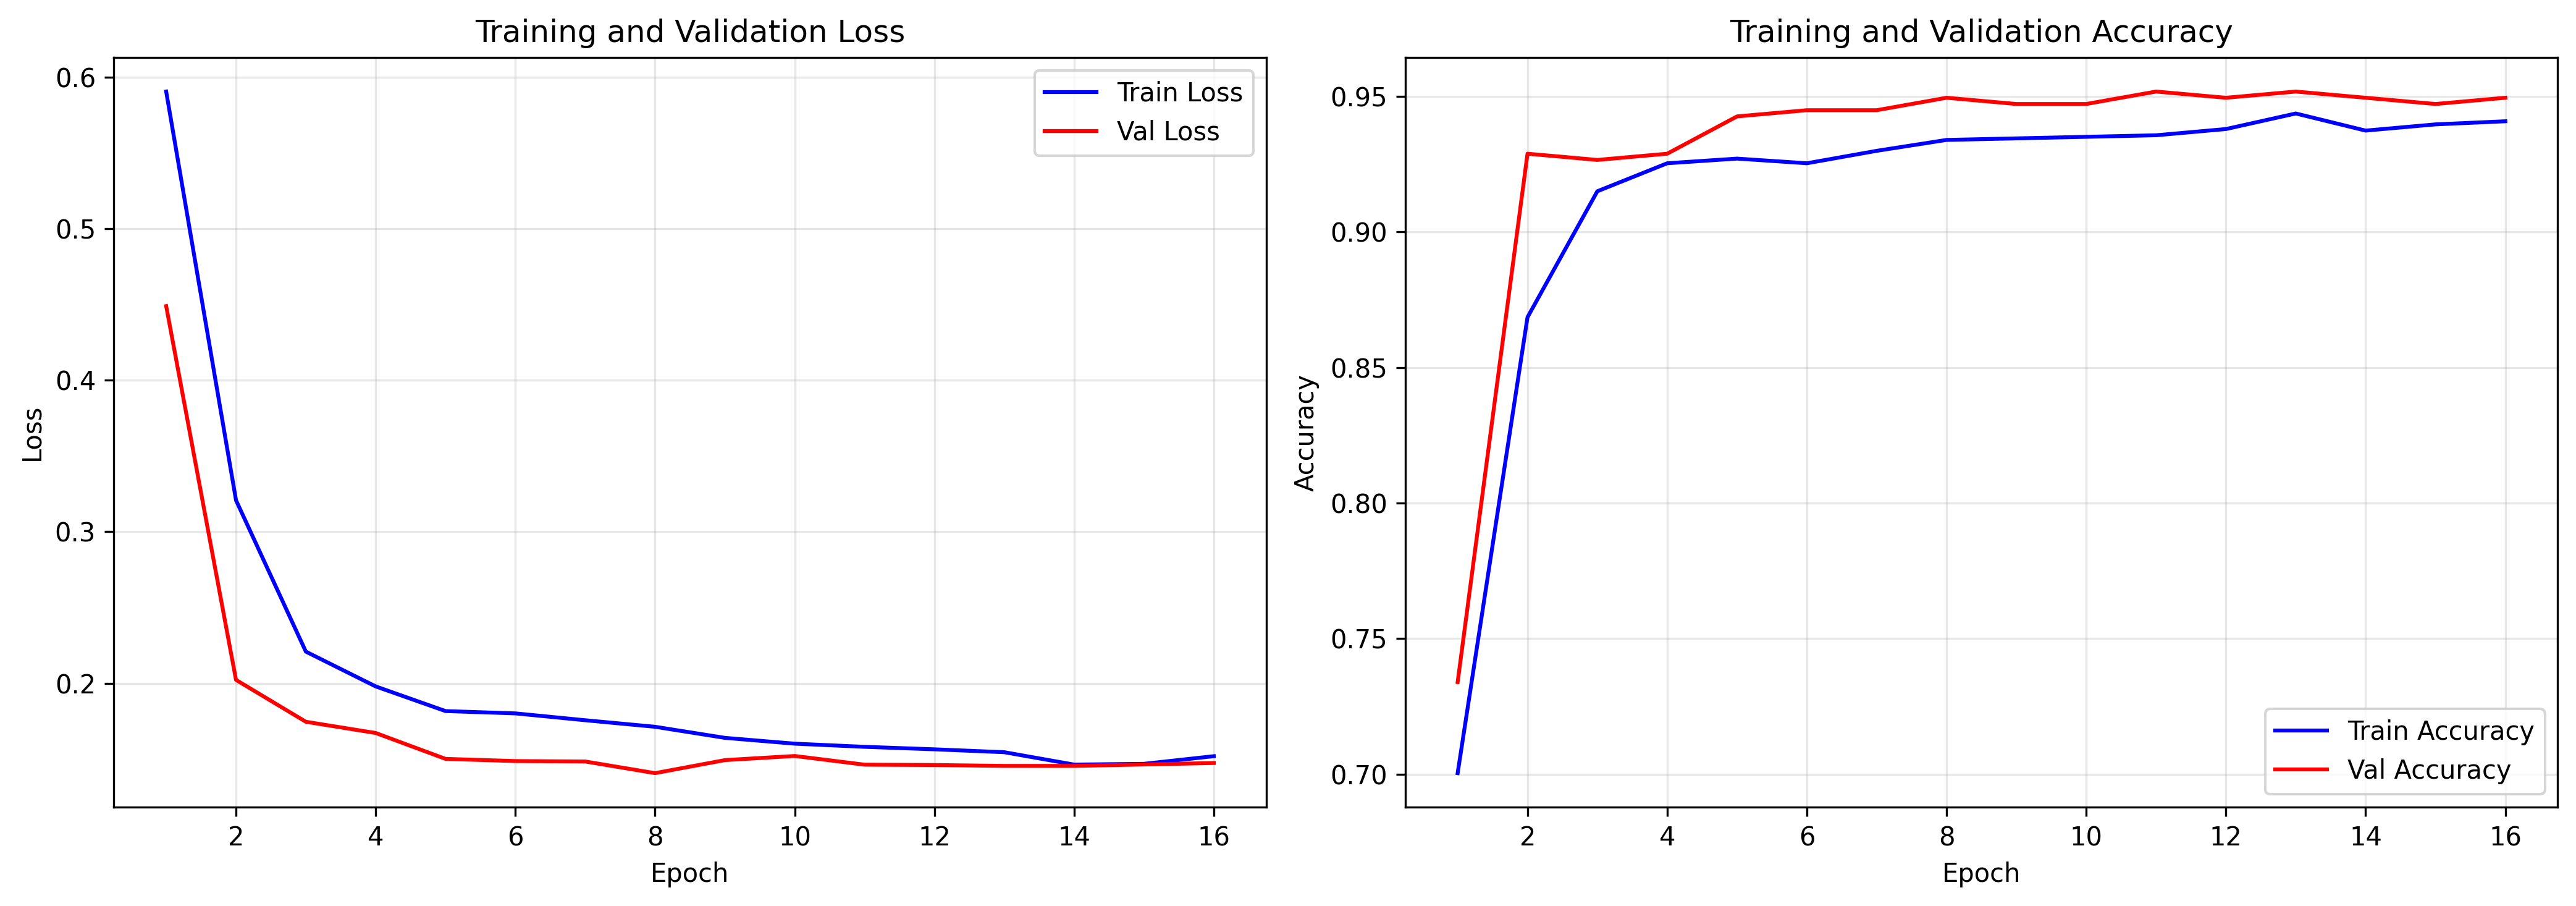
\includegraphics[width=1\textwidth]{figure/training_E4.png}
\caption{Kurva Pelatihan Eksperimen E4 pada Model Unimodal Gambar}
\label{fig:training_E4}
\end{figure} 


Berdasarkan kurva pelatihan pada eksperimen E4 yang dapat dilihat pada Gambar \ref{fig:training_E4}, terlihat bahwa proses pembelajaran berlangsung secara stabil dan konvergen. Pada awal \textit{epoch}, nilai \textit{training loss} dan \textit{validation loss} mengalami penurunan yang signifikan, yang menunjukkan bahwa model dengan cepat mampu mempelajari pola dasar dari data. Seiring bertambahnya \textit{epoch}, penurunan \textit{loss} menjadi lebih gradual hingga mencapai kondisi stabil pada kisaran nilai yang rendah, tanpa adanya fluktuasi yang signifikan. Hal ini menunjukkan bahwa model tidak mengalami \textit{overfitting}, yang juga didukung oleh pola \textit{training accuracy} dan \textit{validation accuracy} yang meningkat secara konsisten dan memiliki selisih yang relatif kecil. Selain itu, nilai \textit{validation accuracy} yang sedikit lebih tinggi dibandingkan \textit{training accuracy} pada beberapa \textit{epoch} mengindikasikan bahwa model memiliki kemampuan generalisasi yang baik terhadap data yang belum pernah dilihat. Secara keseluruhan, kurva ini menunjukkan bahwa konfigurasi \textit{hyperparameter} pada eksperimen E4 mampu menghasilkan proses pelatihan yang optimal dan stabil.

\begin{figure}[H]
\centering
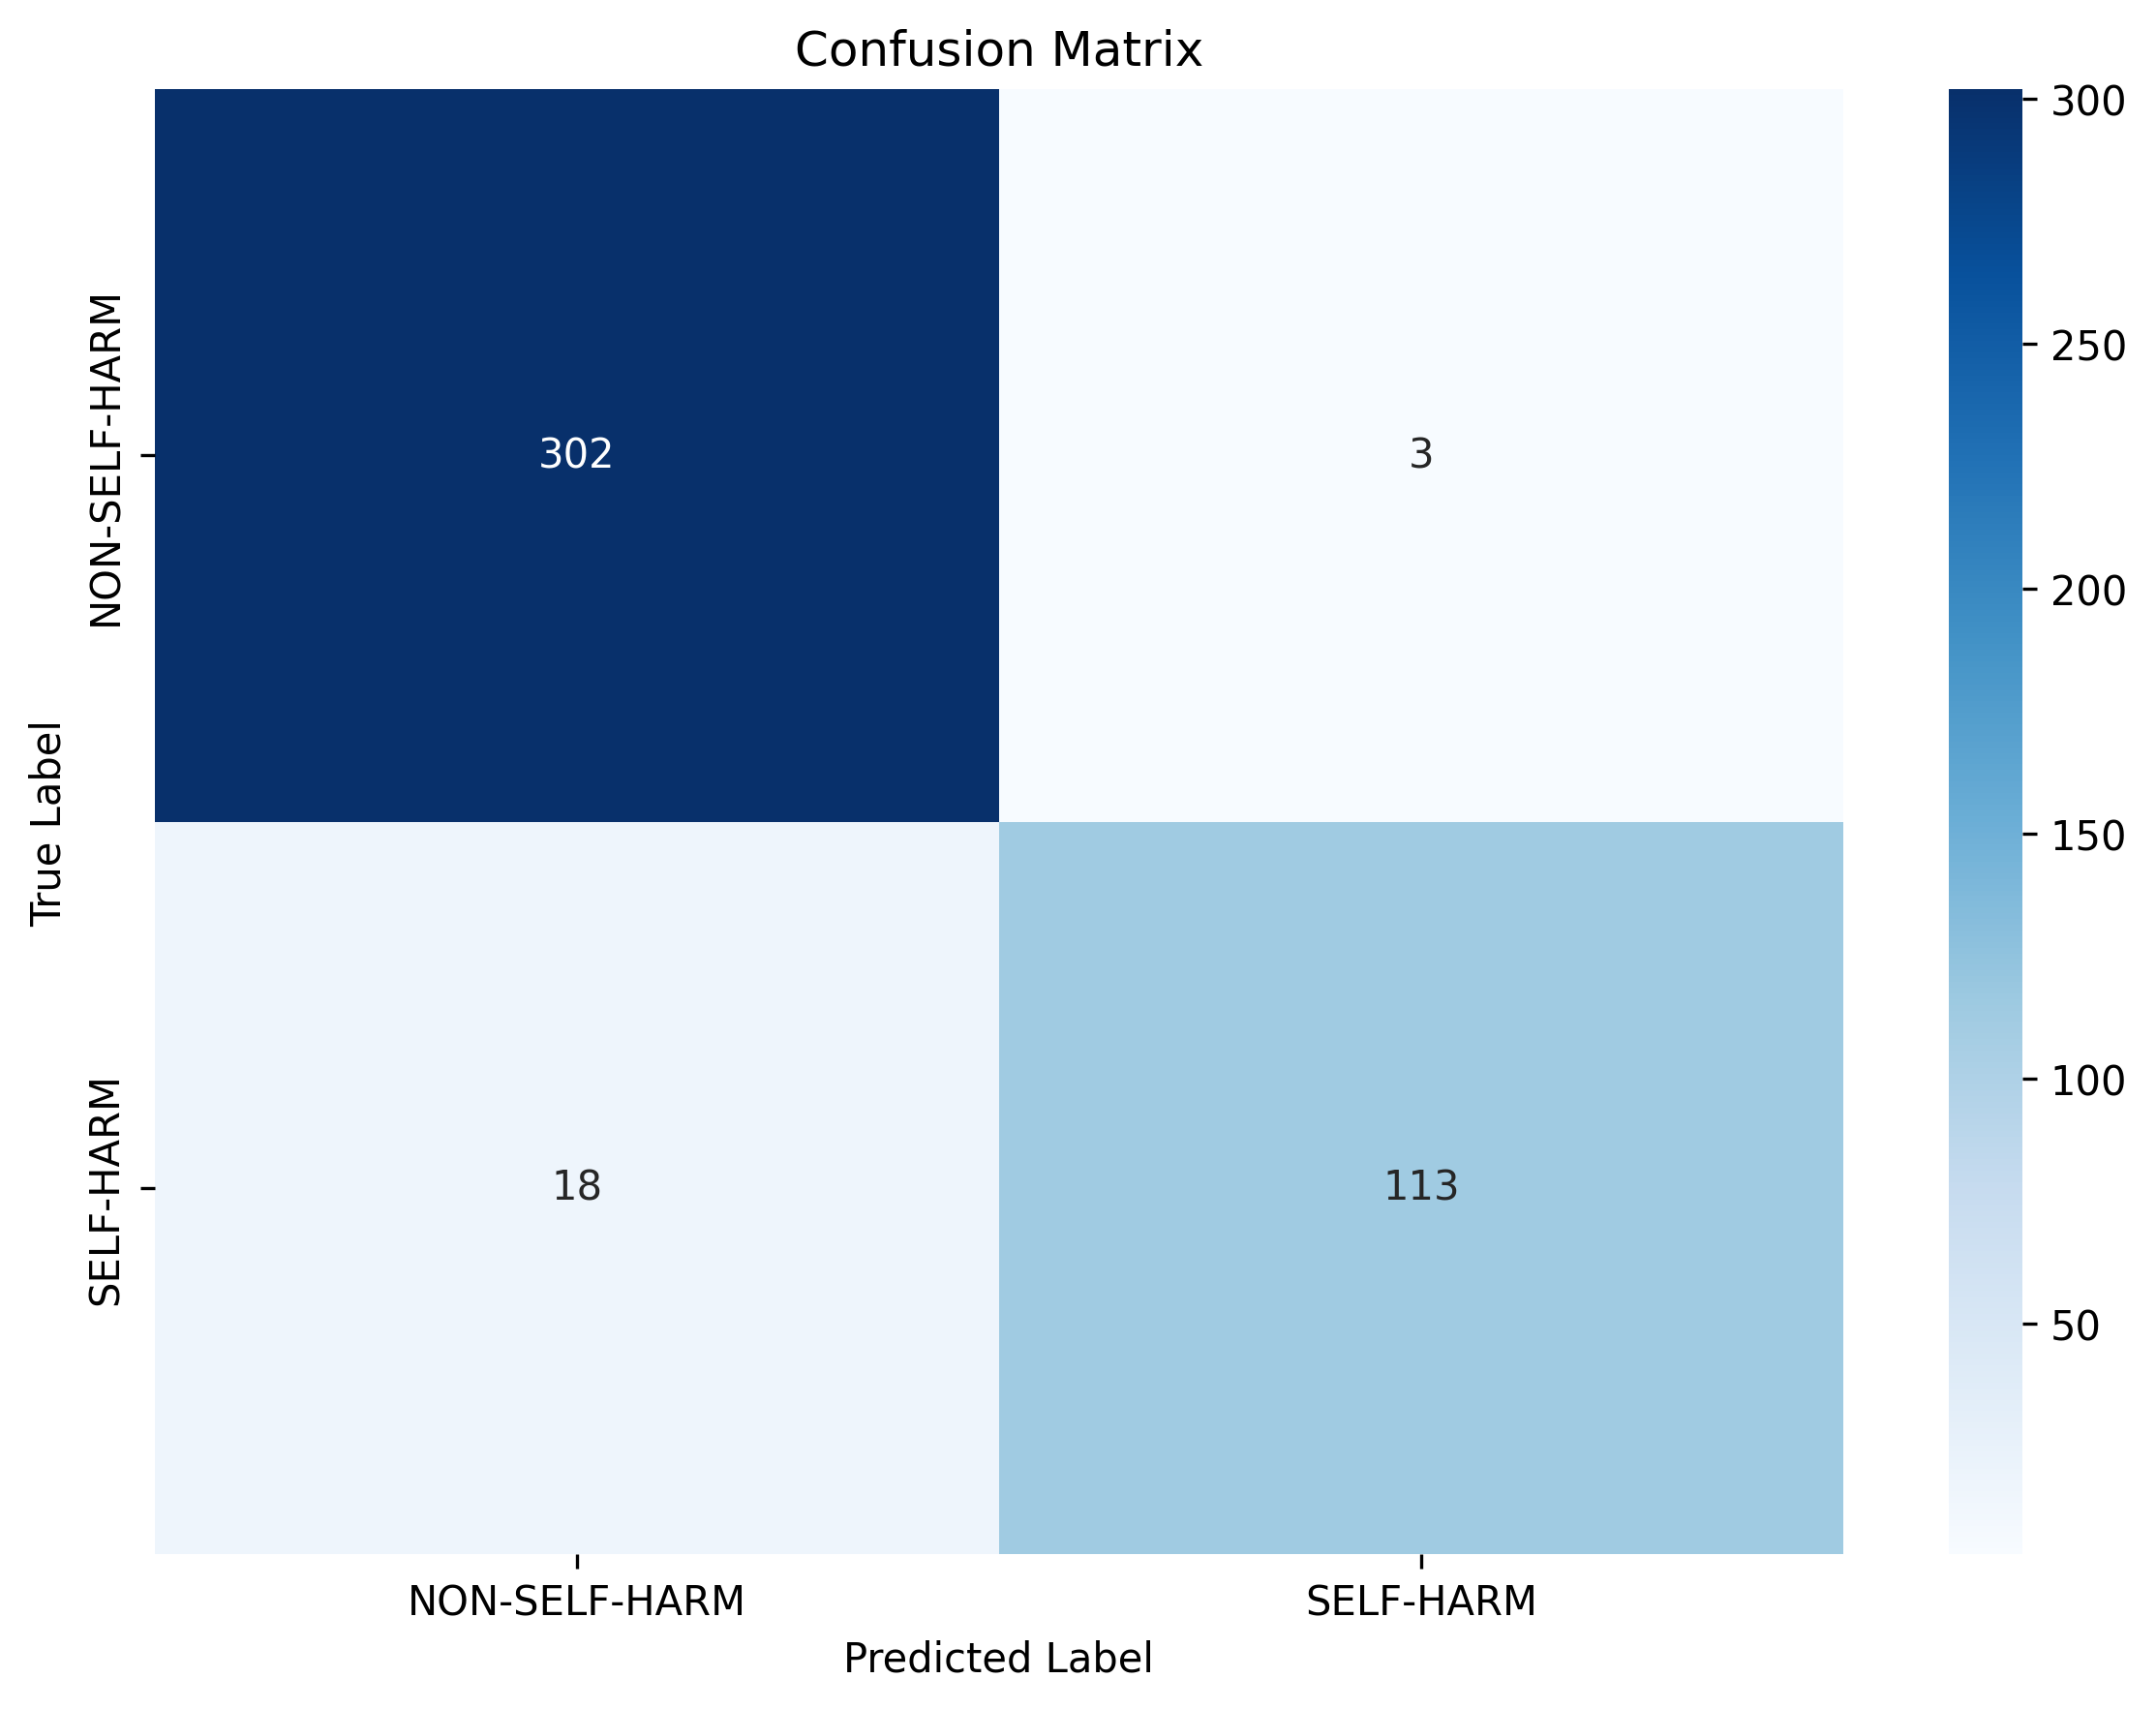
\includegraphics[width=0.5\textwidth]{figure/conf_E4.png}
\caption{\textit{Confusion Matrix} Eksperimen E4 pada Model Unimodal Gambar}
\label{fig:confusion_E4}
\end{figure}

Berdasarkan \textit{confusion matrix} yang dapat dilihat pada Gambar \ref{fig:confusion_E4} , terlihat bahwa model mampu mengklasifikasikan kelas \textit{non-self-harm} dengan sangat baik, ditunjukkan oleh jumlah \textit{true negative} yang tinggi sebanyak 302 data dan hanya 3 kesalahan klasifikasi sebagai \textit{self-harm}. Hal ini menunjukkan bahwa model memiliki kemampuan yang sangat baik dalam mengenali konten non-berbahaya. Namun, pada kelas \textit{self-harm} masih terdapat sejumlah kesalahan, yaitu sebanyak 18 data yang diklasifikasikan sebagai \textit{non-self-harm} (\textit{false negative}), sementara 113 data berhasil terdeteksi dengan benar sebagai \textit{self-harm}. Kondisi ini menunjukkan bahwa meskipun model memiliki \textit{precision} yang tinggi, masih terdapat keterbatasan dalam menangkap seluruh indikasi \textit{self-harm}, terutama yang bersifat implisit dalam representasi visual. Hal ini menunjukkan bahwa modalitas gambar saja belum cukup untuk menangkap seluruh konteks \textit{self-harm}, sehingga diperlukan integrasi dengan modalitas lain pada model multimodal.




% ===============================
% 4.3 Eksperimen Modalitas Teks
% ===============================

\subsection{Hasil Eksperimen Model Unimodal Teks}
\label{IV.Eksperimen.Teks}
Subbab ini membahas hasil eksperimen pada modalitas teks menggunakan model \textit{ELECTRA text encoder}. Evaluasi dilakukan untuk mengetahui pengaruh kombinasi \textit{hyperparameter} terhadap performa model dalam mengklasifikasikan meme \textit{self-harm} berdasarkan informasi tekstual. Variasi eksperimen dilakukan terhadap beberapa \textit{hyperparameter}, yaitu \textit{batch size}, jumlah \textit{epoch}, \textit{learning rate}, dan \textit{patience}, sebagaimana telah dirancang pada Bab III. Hasil eksperimen model unimodal teks disajikan pada Tabel \ref{table:4.teks_eksperimenteks}.

\begin{table}[H]
    \centering
    \caption{Hasil Eksperimen Model unimodal Teks}
    \label{table:4.teks_eksperimenteks}
    \scriptsize
    \setlength{\tabcolsep}{2pt} 
    \renewcommand{\arraystretch}{1.1}
    \resizebox{\textwidth}{!}{%
        \begin{tabular}{ccccccccccccccc}
            \hline
            \textbf{Kode} & \textbf{\textit{Batch}} & \textbf{\textit{Epoch}} & \textbf{\textit{LR}} & \textbf{\textit{Pat.}} & \textbf{\textit{Acc} (\%)} & \textbf{\textit{Prec} (\%)} & \textbf{\textit{Rec} (\%)} & \textbf{\textit{F1} (\%)} & \textbf{TP} & \textbf{TN} & \textbf{FP} & \textbf{FN} & \shortstack{\textbf{Best}\\\textbf{Epc}} & \shortstack{\textbf{Val}\\\textbf{Loss}} \\
            \hline
            \textbf{E6} & \textbf{16} & \textbf{24} & \textbf{1e-4} & \textbf{5} & \textbf{95,4} & \textbf{96,6} & \textbf{87,8} & \textbf{92,0} & \textbf{115} & \textbf{301} & \textbf{4} & \textbf{16} & \textbf{4} & \textbf{0,13} \\
            E7 & 32 & 24 & 1e-5 & 5 & 94,7 & 92,2 & 90,1 & 91,1 & 118 & 295 & 10 & 13 & 1 & 0,47 \\
            E8 & 16 & 12 & 1e-5 & 3 & 94,7 & 92,2 & 90,1 & 91,1 & 118 & 295 & 10 & 13 & 1 & 0,33 \\
            E9 & 8 & 24 & 1e-4 & 5 & 95,2 & 96,6 & 87,0 & 91,6 & 114 & 301 & 4 & 17 & 3 & 0,14 \\
            E10 & 16 & 24 & 1e-6 & 5 & 94,7 & 92,2 & 90,1 & 91,1 & 118 & 295 & 10 & 13 & 2 & 0,62 \\
            \hline
        \end{tabular}
    }
    \smallskip
    \begin{flushleft}
    \footnotesize \textit{Catatan: Baris yang diformat tebal menunjukkan eksperimen dengan performa model terbaik.}
    \end{flushleft}
\end{table}


Berdasarkan hasil eksperimen pada model unimodal teks, terlihat bahwa performa model relatif stabil pada berbagai kombinasi \textit{hyperparameter} dibandingkan dengan model unimodal gambar. Seluruh konfigurasi menunjukkan nilai \textit{accuracy} dan \textit{F1-score} yang cukup tinggi, dengan rentang \textit{F1-score} berada di atas 91\%. Hal ini menunjukkan bahwa representasi tekstual yang dihasilkan oleh ELECTRA mampu menangkap informasi yang relevan dalam mendeteksi konten \textit{self-harm}. Berbeda dengan modalitas gambar, model tidak mengalami kegagalan pembelajaran meskipun menggunakan \textit{learning rate} yang lebih kecil, yang mengindikasikan bahwa fitur tekstual memiliki pola yang lebih eksplisit dan mudah dipelajari oleh model.

Konfigurasi terbaik diperoleh pada eksperimen E6 dengan \textit{batch size} 16, \textit{epoch} 24, \textit{learning rate} 1e-4, dan \textit{patience} 5, yang menghasilkan \textit{accuracy} sebesar 95,4\% dan \textit{F1-score} sebesar 92,0\%. Nilai \textit{precision} yang tinggi (96,6\%) menunjukkan bahwa model mampu mengidentifikasi kelas \textit{self-harm} dengan cukup akurat, sementara nilai \textit{recall} sebesar 87,8\% menunjukkan bahwa sebagian besar kasus \textit{self-harm} berhasil terdeteksi. Meskipun demikian, masih terdapat sejumlah data yang tidak teridentifikasi dengan baik, yang menunjukkan bahwa meskipun modalitas teks lebih informatif dibandingkan gambar, penggunaan satu modalitas saja masih memiliki keterbatasan dalam menangkap keseluruhan konteks meme yang kompleks. Oleh karena itu, integrasi dengan modalitas visual melalui pendekatan multimodal diharapkan dapat meningkatkan performa model secara lebih optimal.
\begin{figure}[H]
\centering
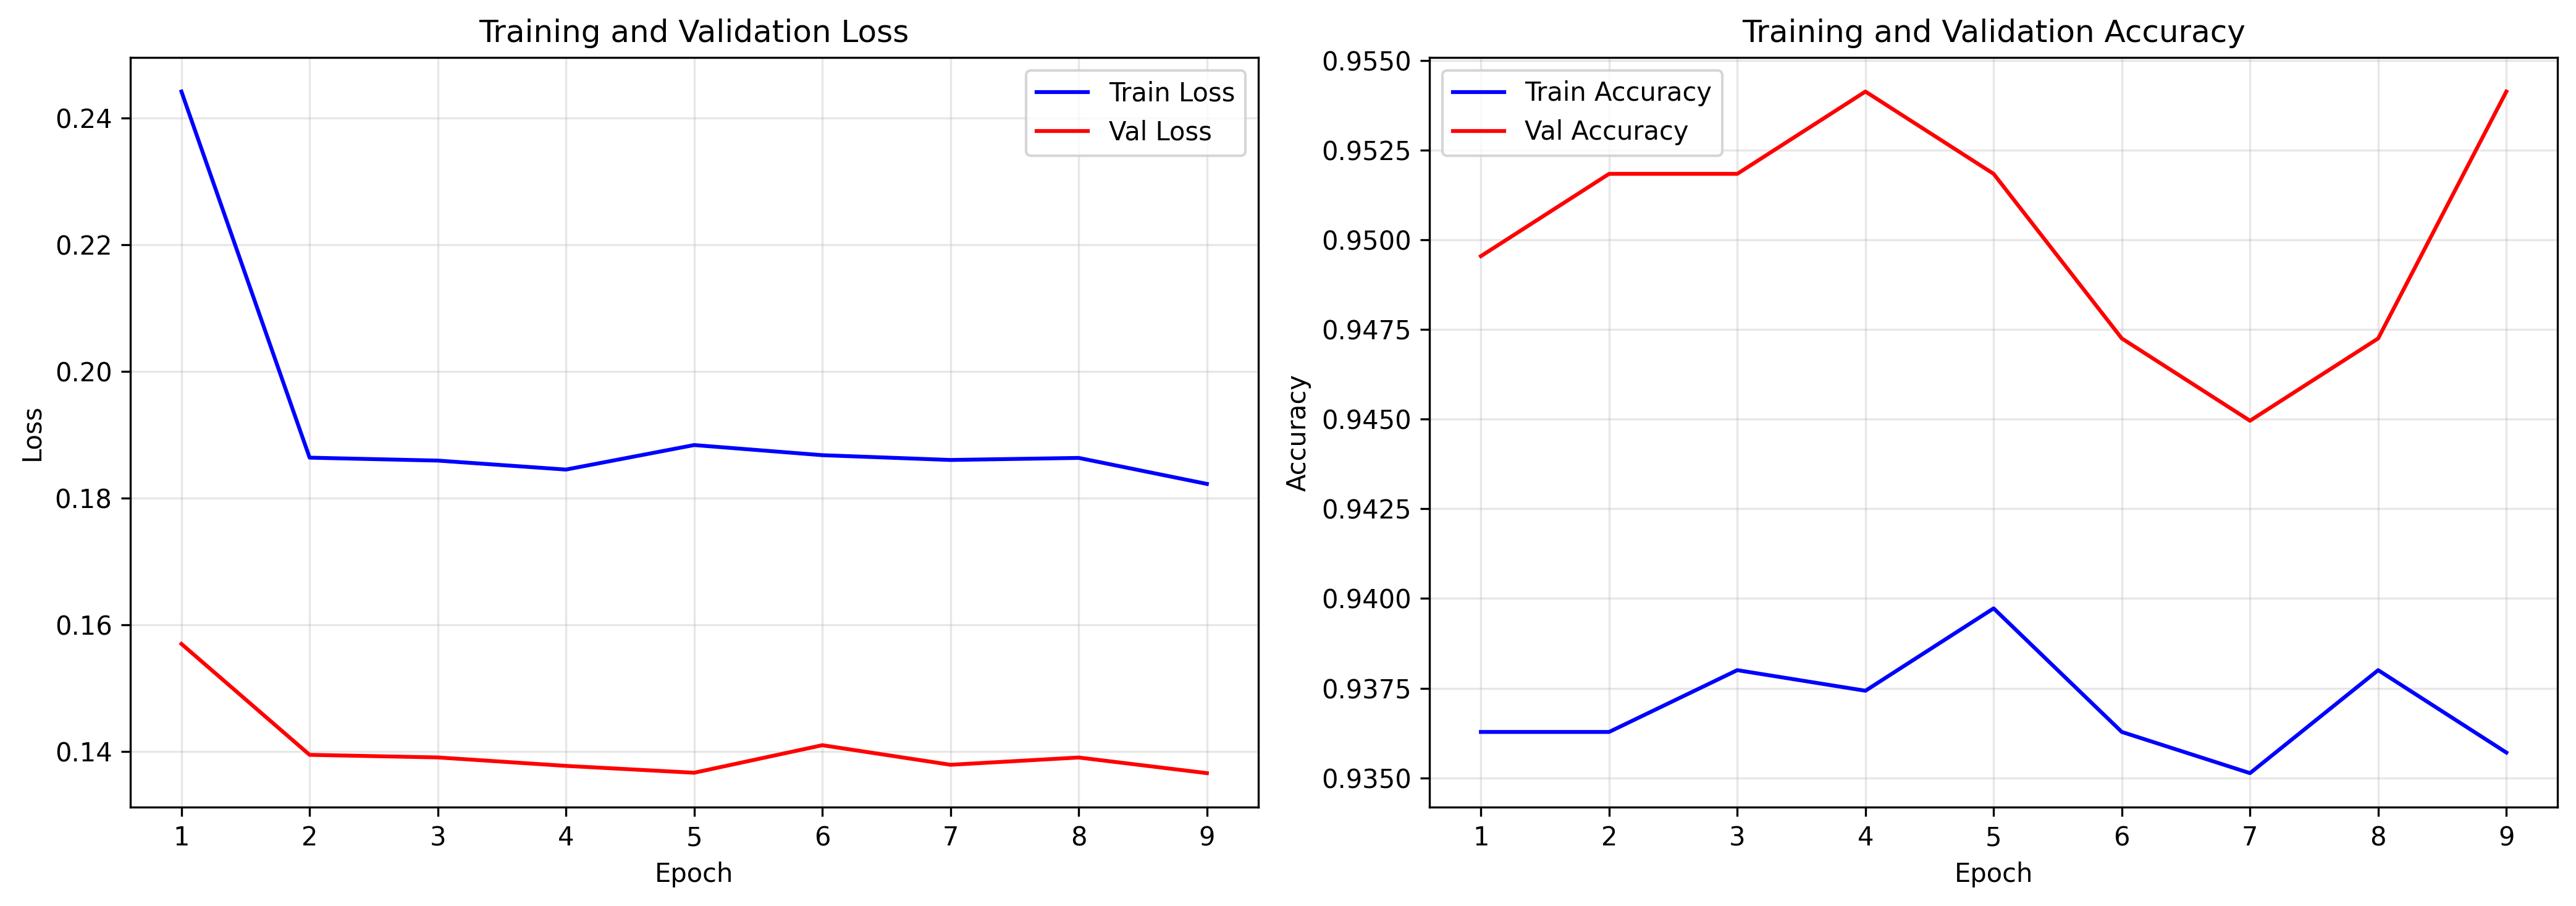
\includegraphics[width=1\textwidth]{figure/training_E6.png}
\caption{Kurva Pelatihan Eksperimen E6 pada Model Unimodal Teks}
\label{fig:training_E6}
\end{figure}

Berdasarkan kurva pelatihan pada eksperimen E6 yang dapat dilihat pada Gambar \ref{fig:training_E6} , terlihat bahwa proses pembelajaran berlangsung stabil sejak awal hingga akhir \textit{epoch}. Nilai \textit{training loss} dan \textit{validation loss} mengalami penurunan yang cukup signifikan pada \textit{epoch} awal, kemudian cenderung stabil dengan fluktuasi yang relatif kecil pada \textit{epoch} berikutnya, yang menunjukkan bahwa model telah mencapai kondisi konvergen. Tidak terdapat perbedaan yang mencolok antara \textit{training loss} dan \textit{validation loss}, sehingga dapat disimpulkan bahwa model tidak mengalami \textit{overfitting}. Hal ini juga didukung oleh kurva \textit{accuracy} yang menunjukkan bahwa \textit{validation accuracy} secara konsisten berada di atas \textit{training accuracy}, dengan selisih yang kecil, yang mengindikasikan kemampuan generalisasi yang baik terhadap data validasi. Meskipun terdapat sedikit fluktuasi pada beberapa \textit{epoch}, secara keseluruhan kurva menunjukkan bahwa konfigurasi \textit{hyperparameter} pada eksperimen E6 mampu menghasilkan proses pelatihan yang stabil dan optimal.

\begin{figure}[H]
\centering
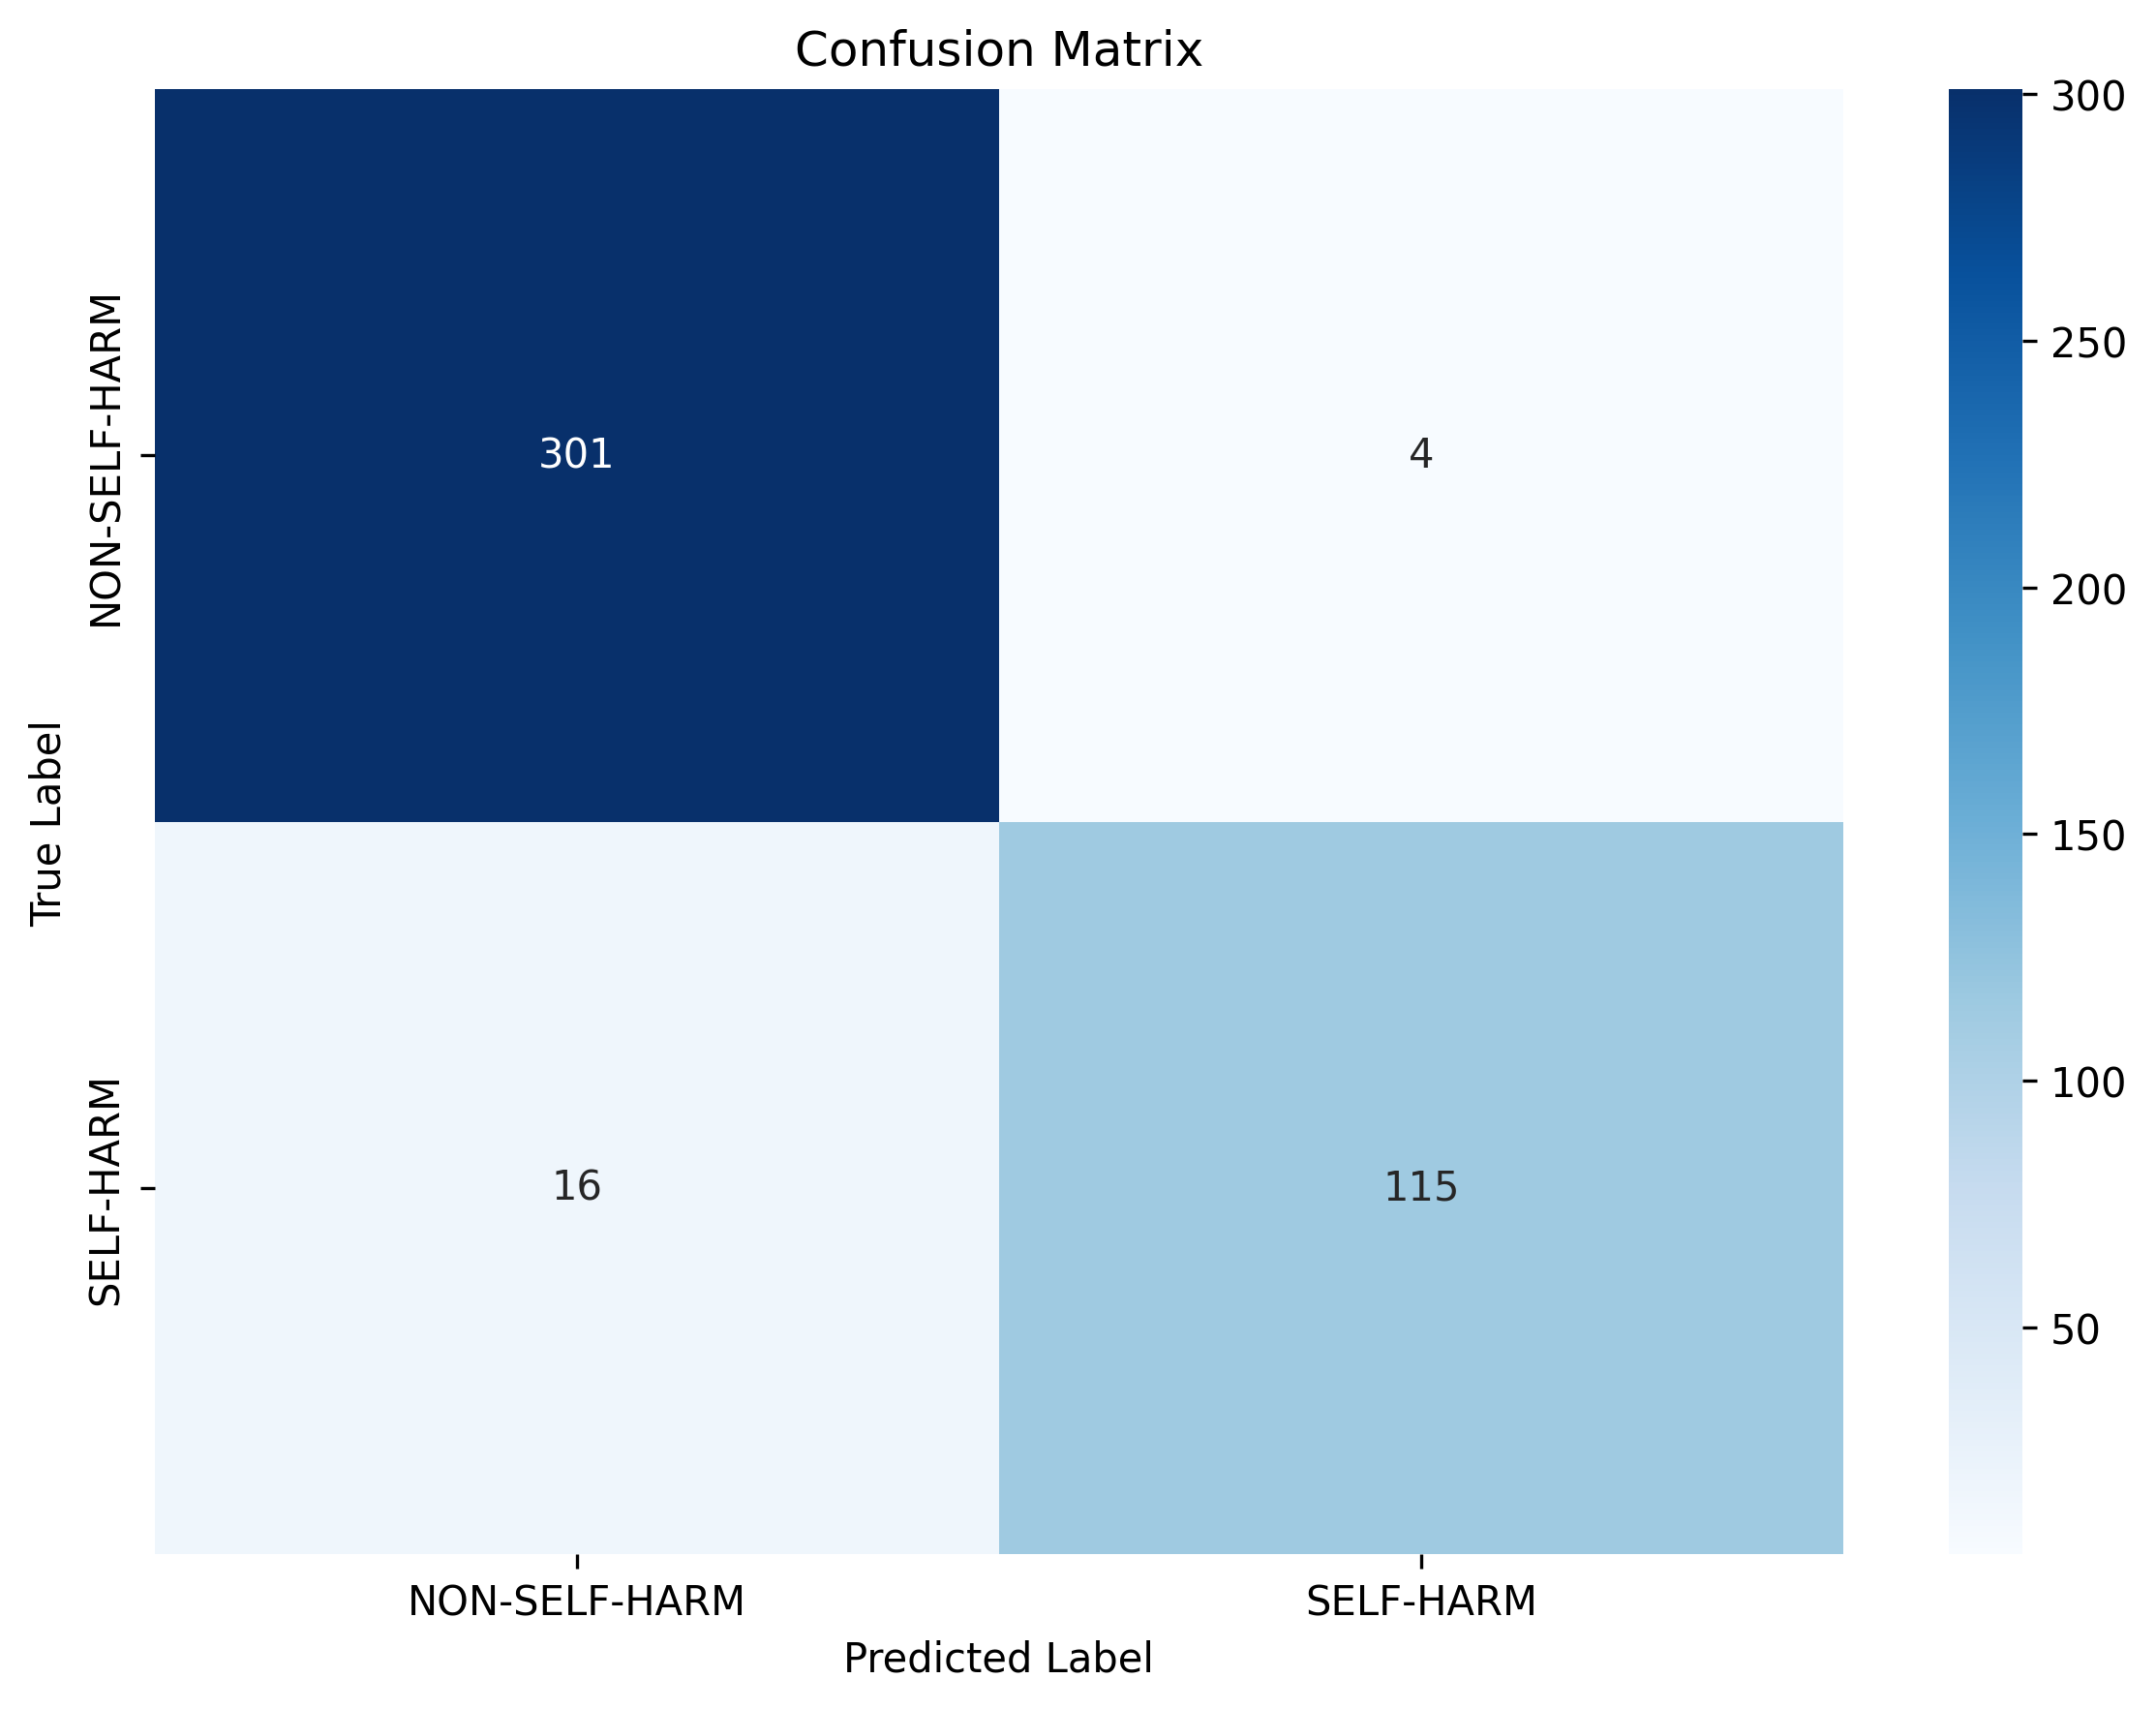
\includegraphics[width=0.5\textwidth]{figure/conf_E6.png}
\caption{\textit{Confusion Matrix} Eksperimen E6 pada Model Unimodal Teks}
\label{fig:confusion_E6}
\end{figure}


Berdasarkan \textit{confusion matrix} pada eksperimen E6, performa model menunjukkan konsistensi dengan nilai metrik evaluasi yang diperoleh, yaitu \textit{precision} sebesar 96,6\%, \textit{recall} sebesar 87,8\%, dan \textit{F1-score} sebesar 92,0\%. Nilai \textit{precision} yang tinggi tercermin dari jumlah \textit{false positive} yang sangat kecil, yaitu hanya 4 data \textit{non-self-harm} yang salah diklasifikasikan sebagai \textit{self-harm}, sehingga model sangat akurat dalam memprediksi kelas positif. Sementara itu, nilai \textit{recall} yang sedikit lebih rendah disebabkan oleh masih adanya 16 data \textit{self-harm} yang tidak terdeteksi (\textit{false negative}), yang menunjukkan bahwa model belum sepenuhnya mampu menangkap seluruh kasus \textit{self-harm}. Kombinasi \textit{precision} dan \textit{recall} tersebut menghasilkan \textit{F1-score} yang tinggi, yang mengindikasikan bahwa model memiliki keseimbangan yang baik dalam performa klasifikasi. Secara keseluruhan, hasil ini menunjukkan bahwa modalitas teks cukup efektif dalam mendeteksi konten \textit{self-harm}, namun masih memiliki keterbatasan dalam menangkap kasus yang bersifat ambigu, sehingga integrasi dengan modalitas visual melalui pendekatan multimodal menjadi penting untuk meningkatkan performa secara lebih optimal.




% =========================================
% 4.x Eksperimen Multimodal
% =========================================

\subsection{Hasil Model Multimodal}
\label{IV.HasilMultimodal}
Subbab ini membahas hasil eksperimen pada model multimodal yang menggabungkan informasi dari modalitas gambar dan teks dalam proses klasifikasi meme \textit{self-harm}. Berbeda dengan pendekatan unimodal, model multimodal diharapkan mampu menangkap hubungan yang lebih kompleks melalui integrasi representasi visual dan tekstual. Evaluasi dilakukan untuk menganalisis pengaruh berbagai konfigurasi eksperimen, termasuk dimensi fitur, strategi \textit{loss}, metode \textit{fusion}, serta pengembangan arsitektur berbasis \textit{Transformer}. Selain itu, subbab ini juga bertujuan untuk membandingkan performa model multimodal dengan model unimodal guna menunjukkan kontribusi integrasi multimodal dalam meningkatkan kinerja klasifikasi.

\subsubsection{Pengaruh Dimensi Fitur}
\label{IV.MultimodalDimensi}
Pada tahap ini, eksperimen dilakukan pada varian model multimodal dengan pendekatan \textit{simple fusion}, di mana representasi fitur teks dan gambar digabungkan secara langsung dan diteruskan ke \textit{MLP classifier}. Untuk memastikan konsistensi evaluasi, kombinasi \textit{hyperparameter} yang digunakan mengacu pada konfigurasi terbaik dari eksperimen model unimodal sebelumnya. Konfigurasi \textit{hyperparameter} ini dipertahankan pada seluruh variasi dimensi fitur, sehingga analisis difokuskan pada pengaruh perubahan dimensi representasi terhadap performa model. Konfigurasi \textit{hyperparameter} yang digunakan adalah sebagai berikut.

\begin{table}[H]
    \centering
    \caption{Konfigurasi \textit{Hyperparameter Training} Model Multimodal Variasi Dimensi}
    \label{table:hyperparams_terpilih}
    \small
    \setlength{\tabcolsep}{3pt}
    \renewcommand{\arraystretch}{1.1}
    \begin{tabular}{p{4.0cm} p{1.5cm}}
        \hline
        \textbf{Parameter} & \textbf{Nilai} \\
        \hline
        \textit{Batch Size} & 16 \\
        \textit{Epochs} & 24 \\
        \textit{Learning Rate} & 1e-4 \\
        \textit{Patience} (\textit{Early Stopping}) & 5 \\
        \hline
    \end{tabular}
\end{table}

Berdasarkan hasil eksperimen variasi dimensi fitur, terlihat bahwa kombinasi dimensi teks dan gambar memiliki pengaruh yang signifikan terhadap performa model multimodal. Secara umum, konfigurasi dengan dimensi yang lebih kecil pada kedua modalitas, yaitu 256 untuk teks dan 256 untuk gambar yaitu pada eksperimen dengan kode E16, menunjukkan performa terbaik dengan \textit{accuracy} sebesar 97,7\% dan \textit{F1-score} sebesar 96,1\%. Hal ini menunjukkan bahwa representasi dengan dimensi yang lebih ringkas mampu menghasilkan fitur yang lebih efektif dan tidak berlebihan, sehingga model dapat mempelajari pola dengan lebih optimal. Sebaliknya, penggunaan dimensi yang lebih besar tidak selalu menghasilkan performa yang lebih baik, yang mengindikasikan adanya kemungkinan redundansi informasi atau \textit{over-representation} pada fitur.

\begin{table}[H]
    \centering
    \caption{Hasil Eksperimen Model multimodal Variasi Dimensi}
    \label{table:4.multimodal_dimensi}
    \scriptsize
    \setlength{\tabcolsep}{2pt}
    \renewcommand{\arraystretch}{1.1}
    \resizebox{\textwidth}{!}{%
        \begin{tabular}{ccccccccccccc}
            \hline
            \textbf{Kode} & \shortstack{\textbf{\textit{Dimensi}}\\\textbf{\textit{Teks}}} & \shortstack{\textbf{\textit{Dimensi}}\\\textbf{\textit{Gambar}}} & \textbf{\textit{Acc} (\%)} & \textbf{\textit{Prec} (\%)} & \textbf{\textit{Rec} (\%)} & \textbf{\textit{F1} (\%)} & \textbf{TP} & \textbf{TN} & \textbf{FP} & \textbf{FN} & \shortstack{\textbf{Best}\\\textbf{Epc}} & \shortstack{\textbf{Val}\\\textbf{Loss}} \\
            \hline
            E11 & 768 & 512 & 97,5 & 98,4 & 93,1 & 95,7 & 122 & 303 & 2 & 9 & 14 & 0,09 \\
            E12 & 768 & 256 & 96,8 & 97,6 & 91,6 & 94,5 & 120 & 302 & 3 & 11 & 6 & 0,10 \\
            E13 & 512 & 512 & 95,4 & 96,6 & 87,8 & 92,0 & 115 & 301 & 4 & 16 & 3 & 0,15 \\
            E14 & 512 & 256 & 97,5 & 98,4 & 93,1 & 95,7 & 122 & 303 & 2 & 9 & 8 & 0,09 \\
            E15 & 256 & 512 & 95,4 & 96,6 & 87,8 & 92,0 & 115 & 301 & 4 & 16 & 2 & 0,14 \\
            \textbf{E16} & \textbf{256} & \textbf{256} & \textbf{97,7} & \textbf{99,2} & \textbf{93,1} & \textbf{96,1} & \textbf{122} & \textbf{304} & \textbf{1} & \textbf{9} & \textbf{7} & \textbf{0,09} \\
            \hline
        \end{tabular}
    }
    \smallskip
    \begin{flushleft}
    \footnotesize \textit{Catatan: Baris yang diformat tebal menunjukkan eksperimen dengan performa model terbaik.}
    \end{flushleft}
\end{table}

Selain itu, terlihat bahwa keseimbangan dimensi antara teks dan gambar juga berperan penting dalam menghasilkan performa yang optimal. Konfigurasi dengan dimensi yang tidak seimbang, seperti E12 (768, 256) atau E15 (256, 512), cenderung menghasilkan performa yang lebih rendah dibandingkan konfigurasi yang seimbang. Hal ini menunjukkan bahwa ketidakseimbangan representasi antar modalitas dapat mempengaruhi proses \textit{fusion}, sehingga interaksi antara fitur teks dan gambar tidak dapat dimodelkan secara optimal. Dengan demikian, hasil eksperimen ini mengindikasikan bahwa pemilihan dimensi fitur yang tepat dan seimbang merupakan faktor penting dalam meningkatkan performa model multimodal berbasis \textit{simple fusion}. Hal ini menunjukkan bahwa peningkatan dimensi tidak selalu berbanding lurus dengan peningkatan performa model.


\begin{figure}[H]
\centering
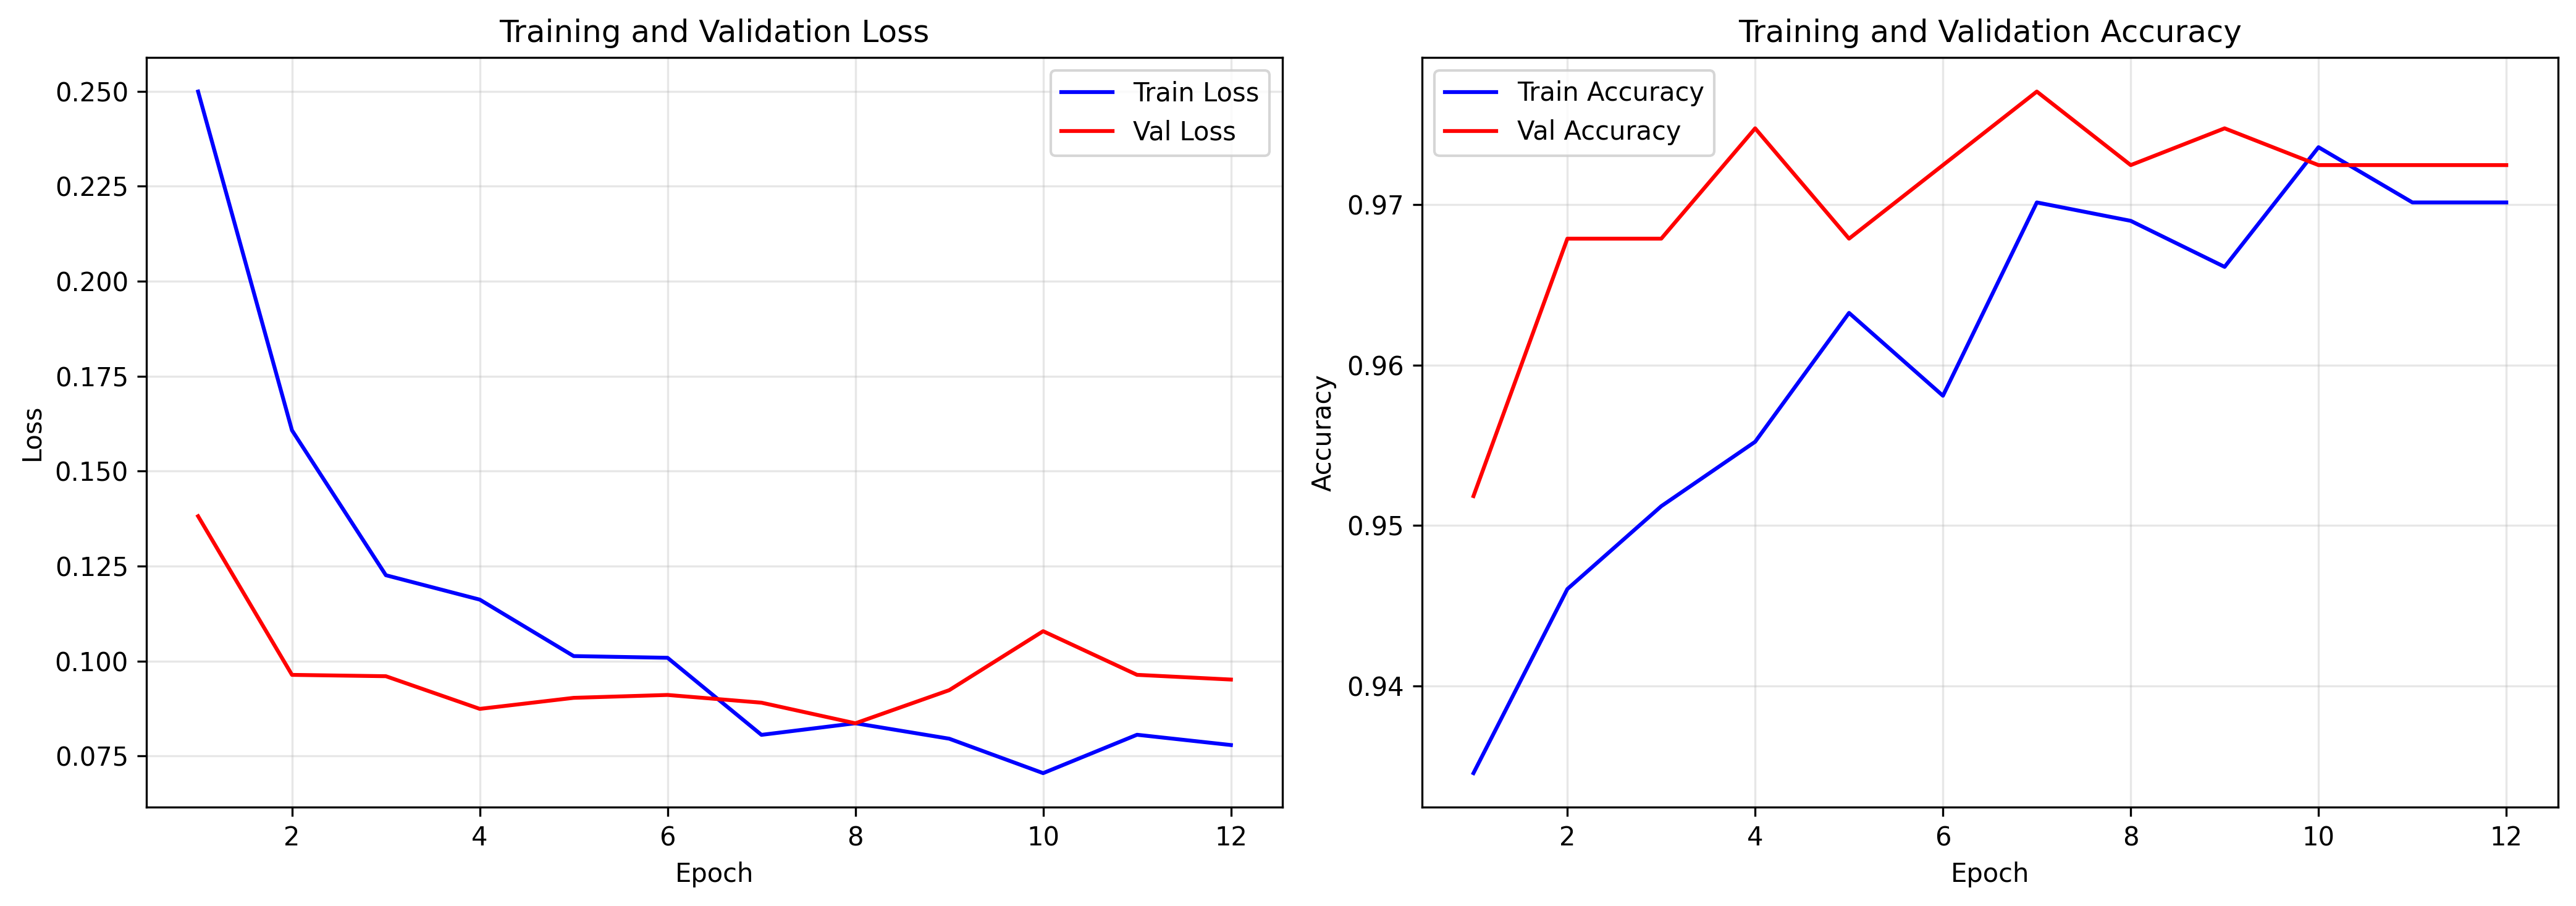
\includegraphics[width=1\textwidth]{figure/training_E16.png}
\caption{Kurva Pelatihan Eksperimen E16 pada Model Multimodal}
\label{fig:training_E16}
\end{figure}

Berdasarkan kurva pelatihan pada eksperimen E16 pada Gambar \ref{fig:training_E16}, terlihat bahwa proses pembelajaran berlangsung dengan baik dan menunjukkan pola konvergensi yang stabil. Pada awal \textit{epoch}, nilai \textit{training loss} dan \textit{validation loss} mengalami penurunan yang cukup signifikan, menandakan bahwa model mampu dengan cepat mempelajari pola dasar dari data. Seiring bertambahnya \textit{epoch}, penurunan \textit{loss} menjadi lebih landai dan cenderung stabil, meskipun terdapat sedikit fluktuasi pada \textit{validation loss} di beberapa \textit{epoch}, yang masih berada dalam batas wajar. Kurva \textit{accuracy} juga menunjukkan peningkatan yang konsisten, dengan \textit{validation accuracy} cenderung lebih tinggi dibandingkan \textit{training accuracy}, yang mengindikasikan bahwa model memiliki kemampuan generalisasi yang baik dan tidak mengalami \textit{overfitting}. Secara keseluruhan, kurva ini menunjukkan bahwa konfigurasi dimensi pada eksperimen E16 mampu menghasilkan proses pelatihan yang optimal dan stabil dalam model multimodal.

\begin{figure}[H]
\centering
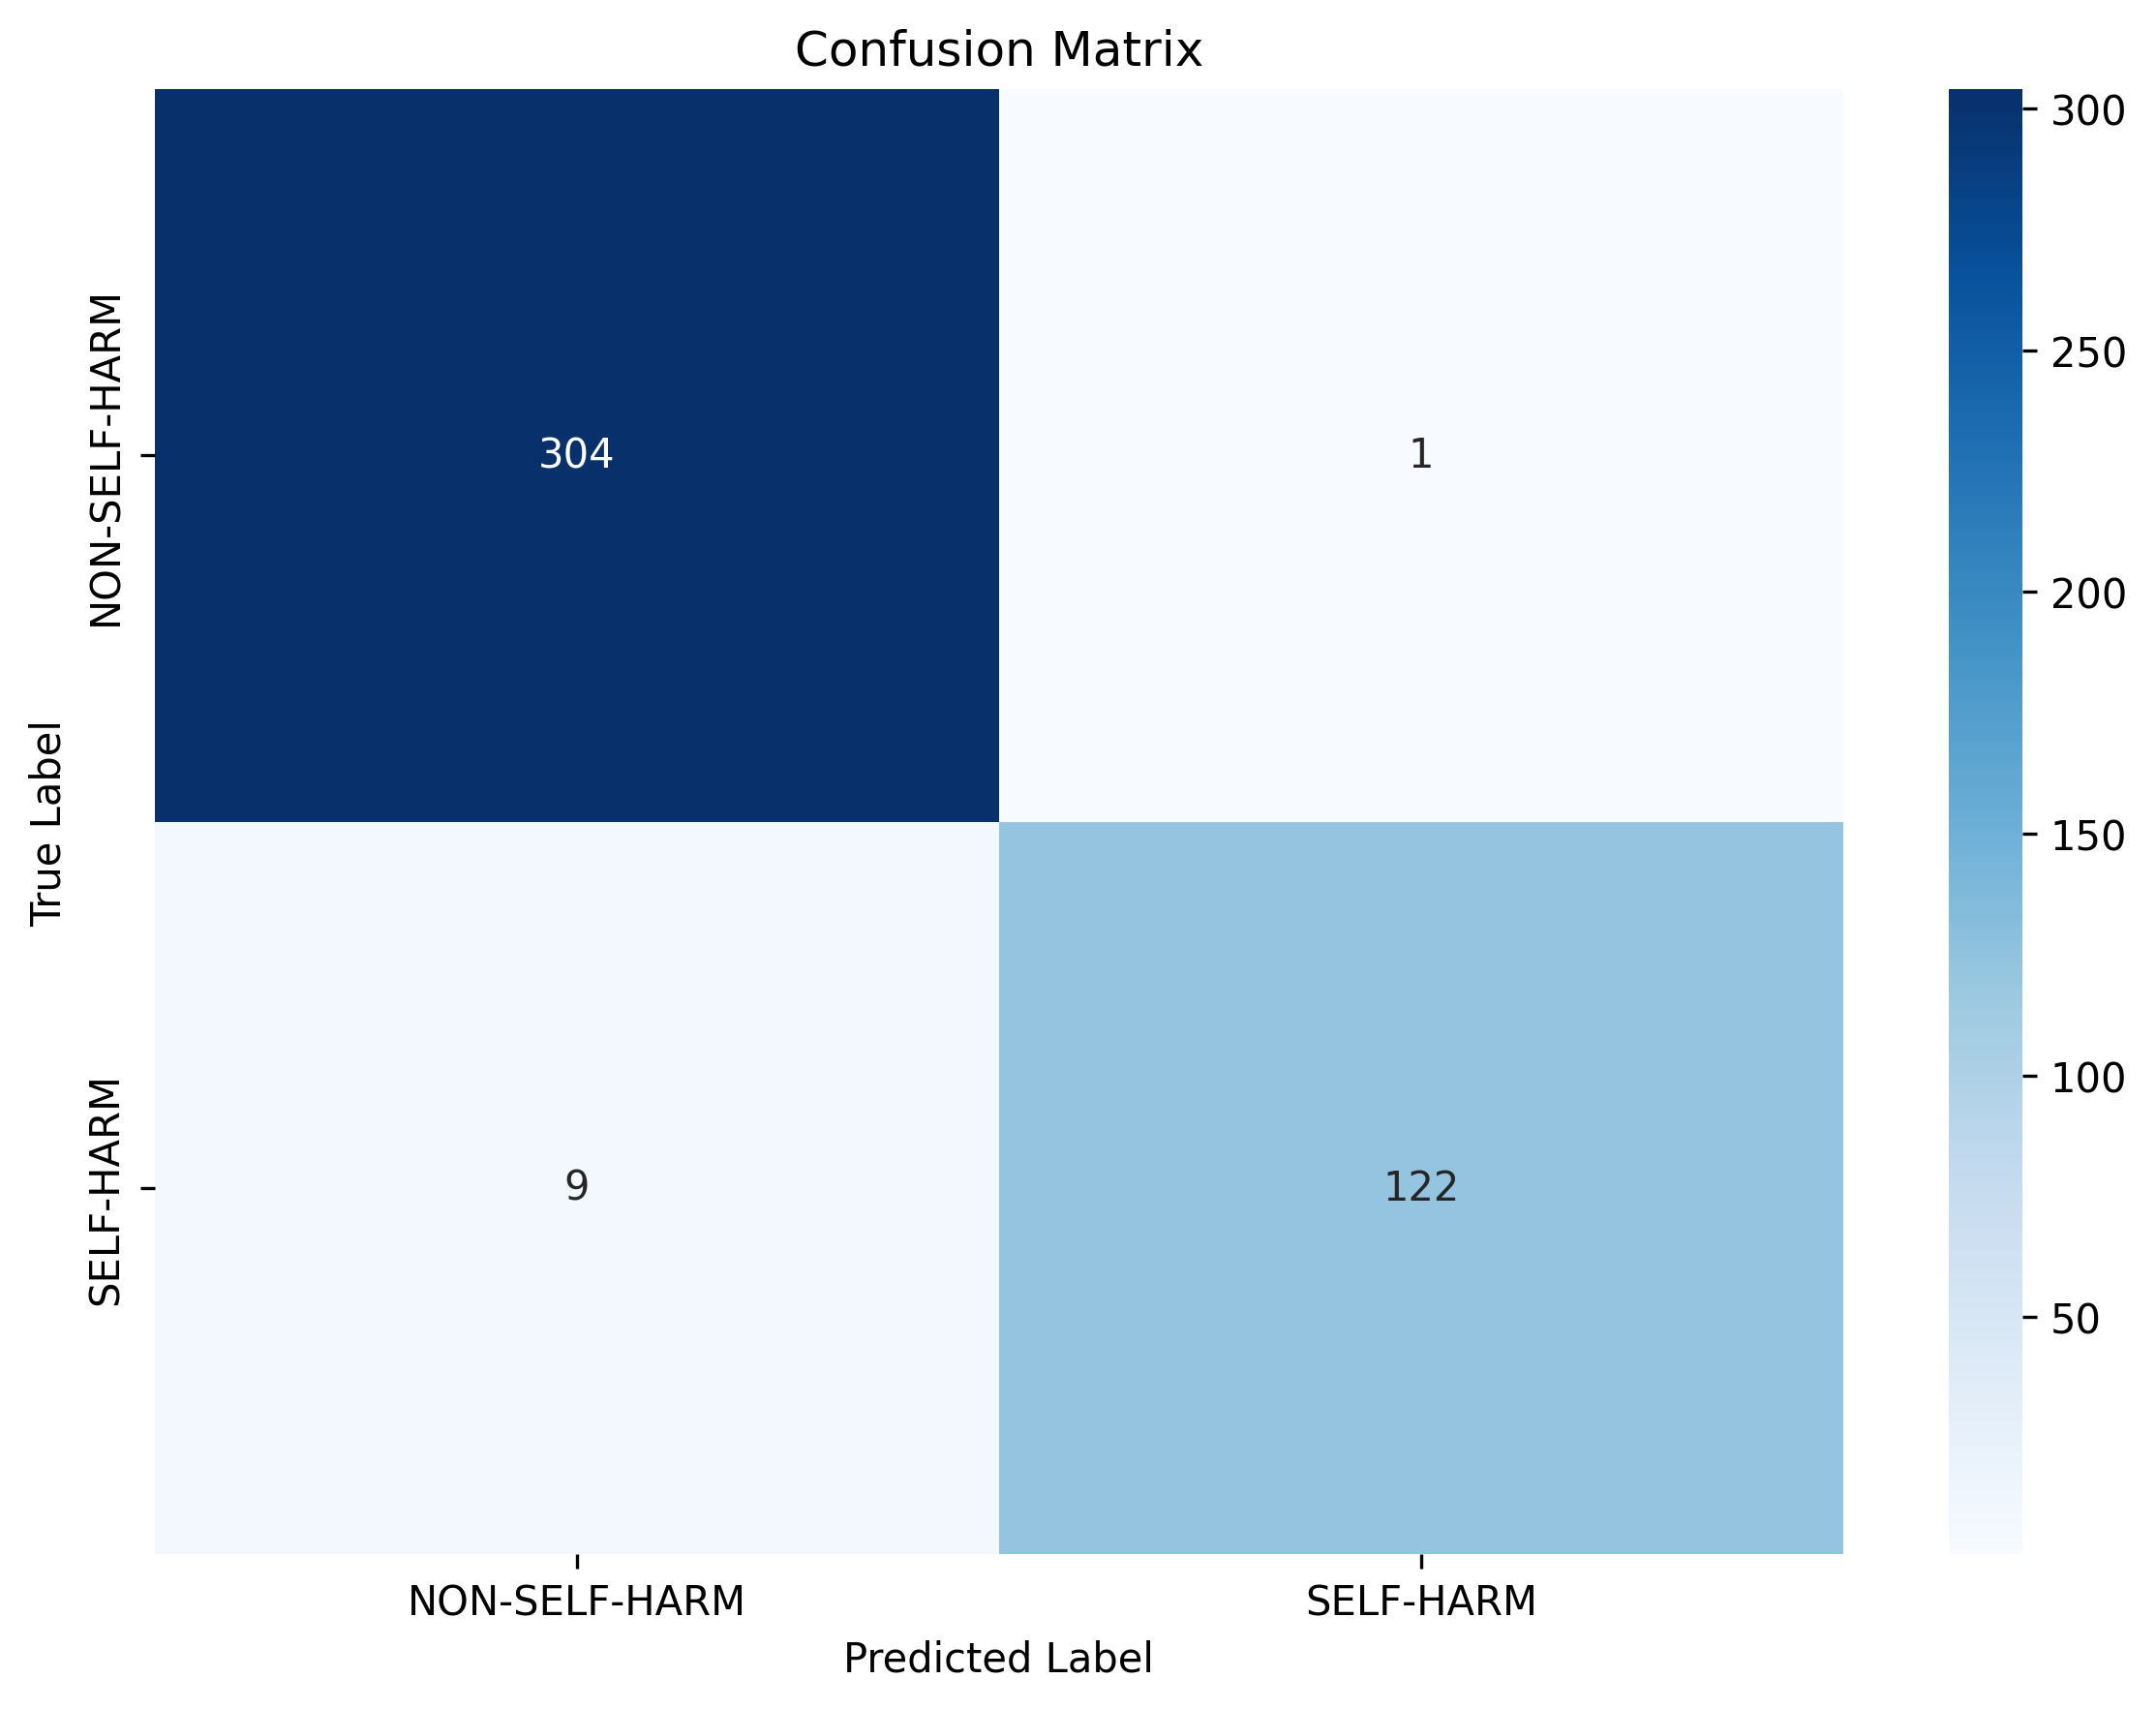
\includegraphics[width=0.5\textwidth]{figure/conf_E16.png}
\caption{\textit{Confusion Matrix} Eksperimen E16 pada Model Multimodal}
\label{fig:confusion_E16}
\end{figure}


Berdasarkan \textit{confusion matrix} pada eksperimen E16 yang dapat dilihat pada Gambar \ref{fig:confusion_E16}, terlihat bahwa model memiliki performa yang sangat baik dan konsisten dengan nilai metrik evaluasi yang diperoleh, yaitu \textit{accuracy} sebesar 97,7\%, \textit{precision} 99,2\%, \textit{recall} 93,1\%, dan \textit{F1-score} 96,1\%. Nilai \textit{precision} yang sangat tinggi tercermin dari jumlah \textit{false positive} yang sangat kecil, yaitu hanya 1 data \textit{non-self-harm} yang salah diklasifikasikan sebagai \textit{self-harm}, sehingga model sangat akurat dalam memprediksi kelas positif. Sementara itu, nilai \textit{recall} yang tinggi namun tidak sempurna disebabkan oleh masih adanya 9 data \textit{self-harm} yang tidak terdeteksi (\textit{false negative}), yang menunjukkan bahwa meskipun model sudah sangat baik, masih terdapat beberapa kasus yang sulit dikenali. Jumlah \textit{true positive} yang tinggi (122 data) menunjukkan kemampuan model dalam mendeteksi sebagian besar konten \textit{self-harm} dengan tepat. Kombinasi \textit{precision} dan \textit{recall} tersebut menghasilkan \textit{F1-score} yang tinggi, yang mengindikasikan keseimbangan performa klasifikasi yang optimal. Secara keseluruhan, hasil ini menunjukkan bahwa penggunaan dimensi fitur yang lebih kecil dan seimbang pada kedua modalitas mampu meningkatkan efektivitas model multimodal dalam menangkap hubungan antar-modalitas dibandingkan konfigurasi lainnya. Temuan ini selanjutnya digunakan sebagai dasar dalam eksperimen berikutnya pada strategi \textit{loss} untuk model multimodal.




\subsubsection{Pengaruh Strategi \textit{Loss}}
\label{IV.MultimodalLoss}
Pada tahap ini, eksperimen dilakukan untuk menganalisis pengaruh strategi \textit{loss} dalam mengatasi permasalahan ketidakseimbangan kelas (\textit{class imbalance}) pada model multimodal. Dataset yang digunakan memiliki distribusi yang tidak seimbang, sebagaimana telah ditunjukkan pada Tabel \ref{table:4.distribusi_label}, di mana kelas \textit{non-self-harm} mendominasi sekitar 70\% dari keseluruhan data, sementara sisanya merupakan kelas \textit{self-harm}. Eksperimen ini menggunakan varian model multimodal dengan pendekatan \textit{simple fusion} yang menggabungkan fitur teks dan gambar sebelum diteruskan ke \textit{MLP classifier}. Untuk menjaga konsistensi evaluasi, konfigurasi \textit{hyperparameter} pelatihan yang digunakan sama seperti pada Tabel \ref{table:hyperparams_terpilih}, dengan menggunakan dimensi terbaik hasil eksperimen sebelumnya, yaitu 256 untuk teks dan 256 untuk gambar.

Berdasarkan hasil eksperimen strategi \textit{loss}, terlihat bahwa penggunaan teknik penanganan \textit{class imbalance} memberikan pengaruh terhadap performa model, khususnya pada metrik \textit{recall} dan \textit{F1-score}. Eksperimen dengan kode E17 dengan metode \textit{Class Weight} mampu meningkatkan sensitivitas model terhadap kelas minoritas dengan menghasilkan \textit{recall} sebesar 93,9\% dan \textit{F1-score} sebesar 95,7\%. Namun, peningkatan ini masih terbatas karena model belum sepenuhnya mampu memfokuskan pembelajaran pada sampel yang sulit. Sementara itu, eksperimen E19 yang menggunakan kombinasi \textit{Class Weight} dan \textit{Focal Loss} menghasilkan \textit{recall} tertinggi sebesar 96,2\%, namun diikuti dengan penurunan \textit{precision} menjadi 94,7\%, yang menunjukkan adanya peningkatan \textit{false positive}. Hal ini menunjukkan adanya \textit{trade-off} antara \textit{precision} dan \textit{recall} dalam penanganan \textit{class imbalance}.

\begin{table}[H]
    \centering
    \caption{Hasil Eksperimen Model Multimodal Strategi Penanganan \textit{Class Imbalance}}
    \label{table:4.multimodal_loss}
    \scriptsize
    \setlength{\tabcolsep}{2pt}
    \renewcommand{\arraystretch}{1.1}
    \resizebox{\textwidth}{!}{%
        \begin{tabular}{l>{\raggedright\arraybackslash}p{2.5cm}cccccccccc}
            \hline
            \textbf{Kode} & \textbf{\textit{Strategy Loss}} & \textbf{\textit{Acc} (\%)} & \textbf{\textit{Prec} (\%)} & \textbf{\textit{Rec} (\%)} & \textbf{\textit{F1} (\%)} & \textbf{TP} & \textbf{TN} & \textbf{FP} & \textbf{FN} & \shortstack{\textbf{Best}\\\textbf{Epc}} & \shortstack{\textbf{Val}\\\textbf{Loss}} \\
            \hline
            E17 & Class Weight (\textit{CELoss}) & 97,5 & 97,6 & 93,9 & 95,7 & 123 & 302 & 3 & 8 & 2 & 0,11 \\
            \textbf{E18} & \textbf{\textit{Focal Loss} ($\gamma = 2{,}0$)} & \textbf{97,7} & \textbf{98,4} & \textbf{93,9} & \textbf{96,1} & \textbf{123} & \textbf{303} & \textbf{2} & \textbf{8} & \textbf{9} & \textbf{0,03} \\
            E19 & \textit{Class Weight} + \textit{Focal Loss} ($\gamma = 2{,}0$) & 97,2 & 94,7 & 96,2 & 95,5 & 126 & 298 & 7 & 5 & 6 & 0,04 \\
            \hline
        \end{tabular}
    }
    \smallskip
    \begin{flushleft}
    \footnotesize \textit{Catatan: Baris yang diformat tebal menunjukkan eksperimen dengan performa model terbaik.}
    \end{flushleft}
\end{table}

Eksperimen E18 dengan metode \textit{Focal Loss} memberikan performa terbaik secara keseluruhan dengan \textit{accuracy} sebesar 97,7\% dan \textit{F1-score} sebesar 96,1\%. \textit{Focal Loss} mampu menyeimbangkan \textit{precision} sebesar 98,4\% dan \textit{recall} sebesar 93,9\% dengan baik, sehingga menghasilkan performa yang lebih stabil dibandingkan metode lainnya. Hal ini menunjukkan bahwa mekanisme \textit{Focal Loss} efektif dalam memfokuskan pembelajaran pada sampel yang sulit tanpa mengorbankan akurasi keseluruhan. Oleh karena itu, strategi \textit{Focal Loss} pada eksperimen E18 dipilih sebagai konfigurasi terbaik dalam menangani ketidakseimbangan kelas pada model multimodal. 
\begin{figure}[H]
\centering
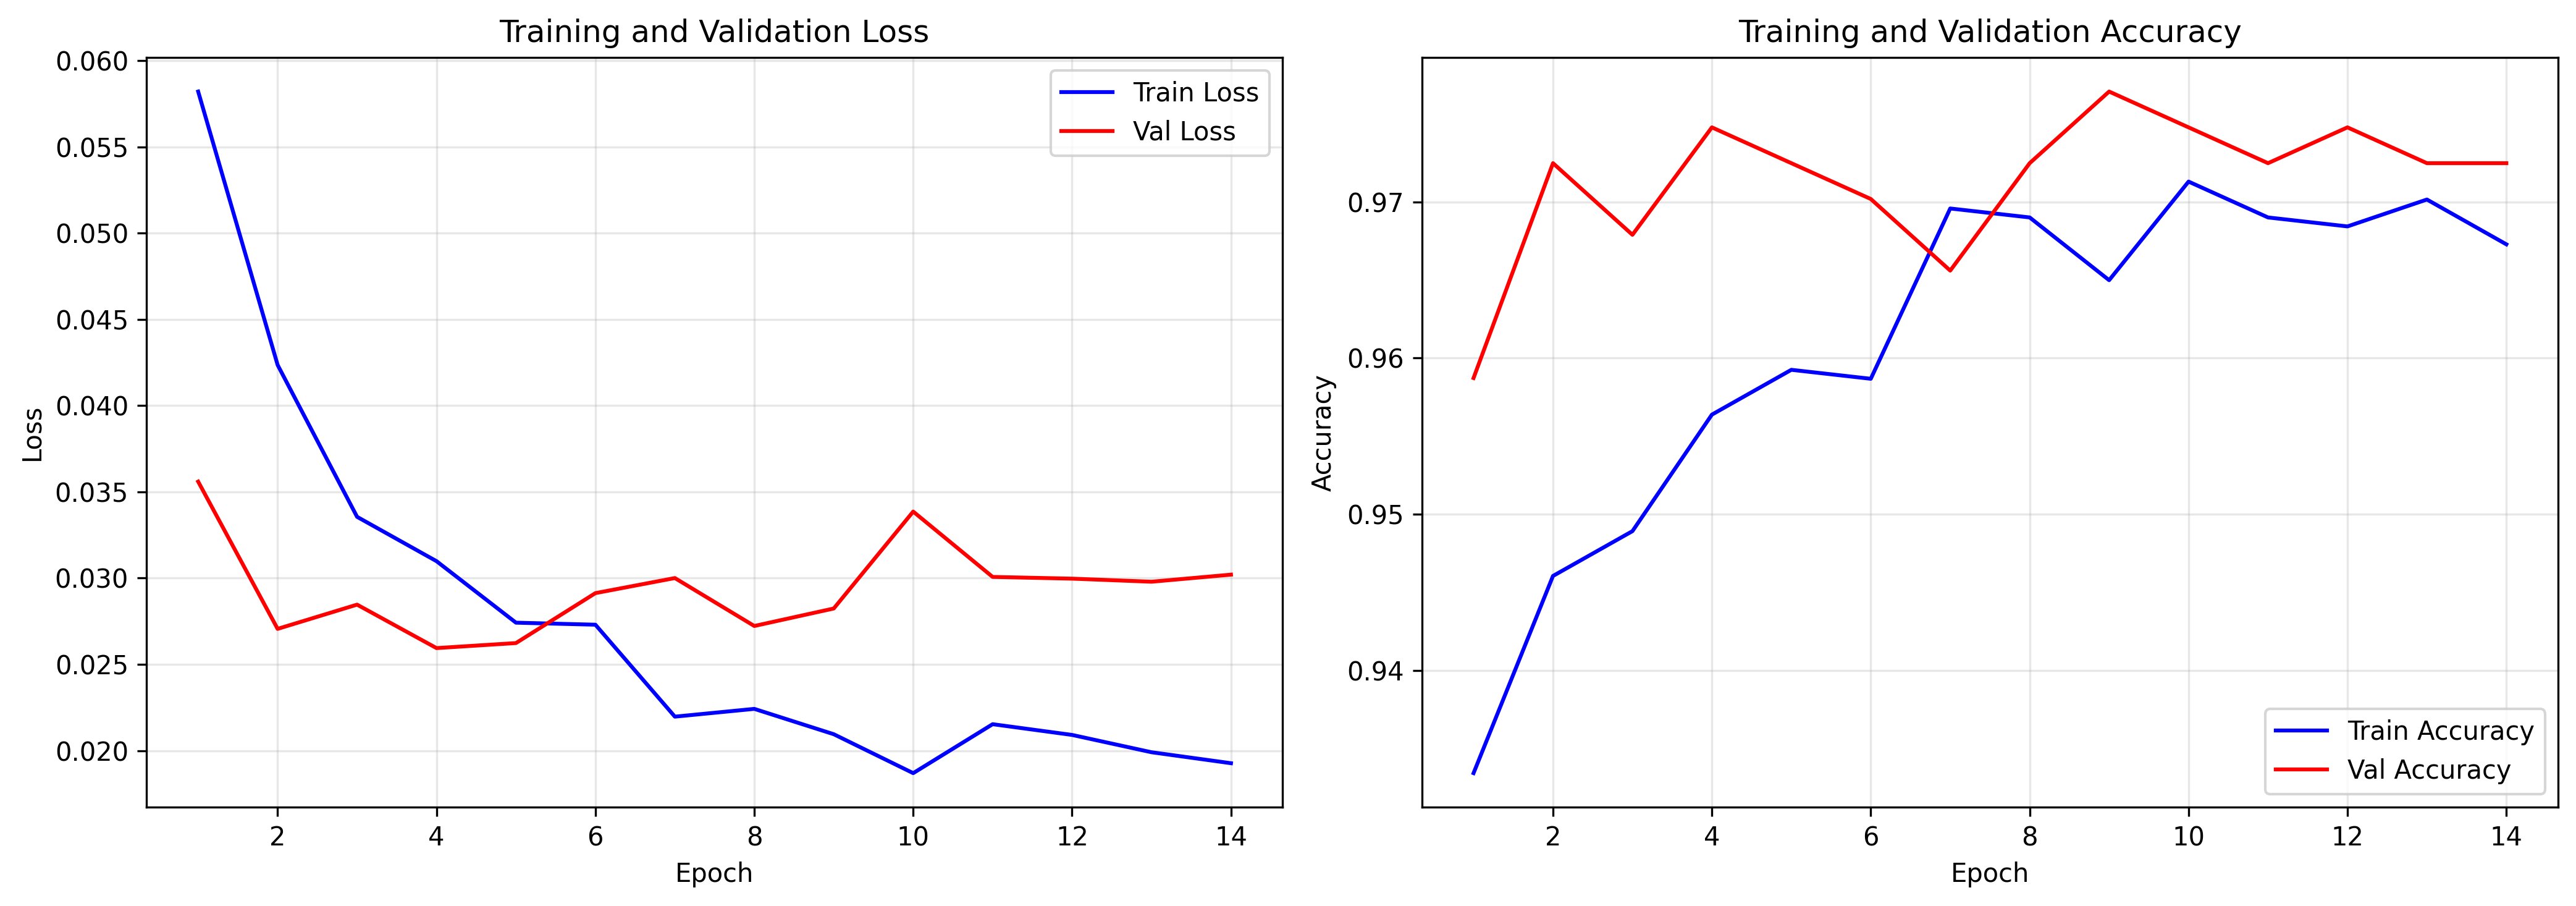
\includegraphics[width=1\textwidth]{figure/training_E18.png}
\caption{Kurva Pelatihan Eksperimen E18 pada Model Multimodal Gambar}
\label{fig:training_E18}
\end{figure}

Berdasarkan kurva pelatihan pada eksperimen 18 pada Gambar \ref{fig:training_E18}, terlihat bahwa proses pembelajaran berlangsung dengan stabil dan menunjukkan konvergensi yang baik. Nilai \textit{training loss} mengalami penurunan yang signifikan pada \textit{epoch} awal dan terus menurun secara bertahap hingga mencapai nilai yang rendah, sementara \textit{validation loss} relatif stabil meskipun terdapat sedikit fluktuasi pada beberapa \textit{epoch}. Pola ini menunjukkan bahwa model mampu mempelajari pola data dengan baik tanpa mengalami \textit{overfitting} yang signifikan. Hal ini juga didukung oleh kurva \textit{accuracy} yang menunjukkan peningkatan yang konsisten pada \textit{training accuracy}, dengan \textit{validation accuracy} yang cenderung lebih tinggi dan stabil sepanjang proses pelatihan. Secara keseluruhan, kurva ini mengindikasikan bahwa penggunaan \textit{Focal Loss} pada eksperimen 18 mampu menghasilkan proses pelatihan yang optimal serta meningkatkan kemampuan generalisasi model dalam menghadapi ketidakseimbangan kelas.

\begin{figure}[H]
\centering
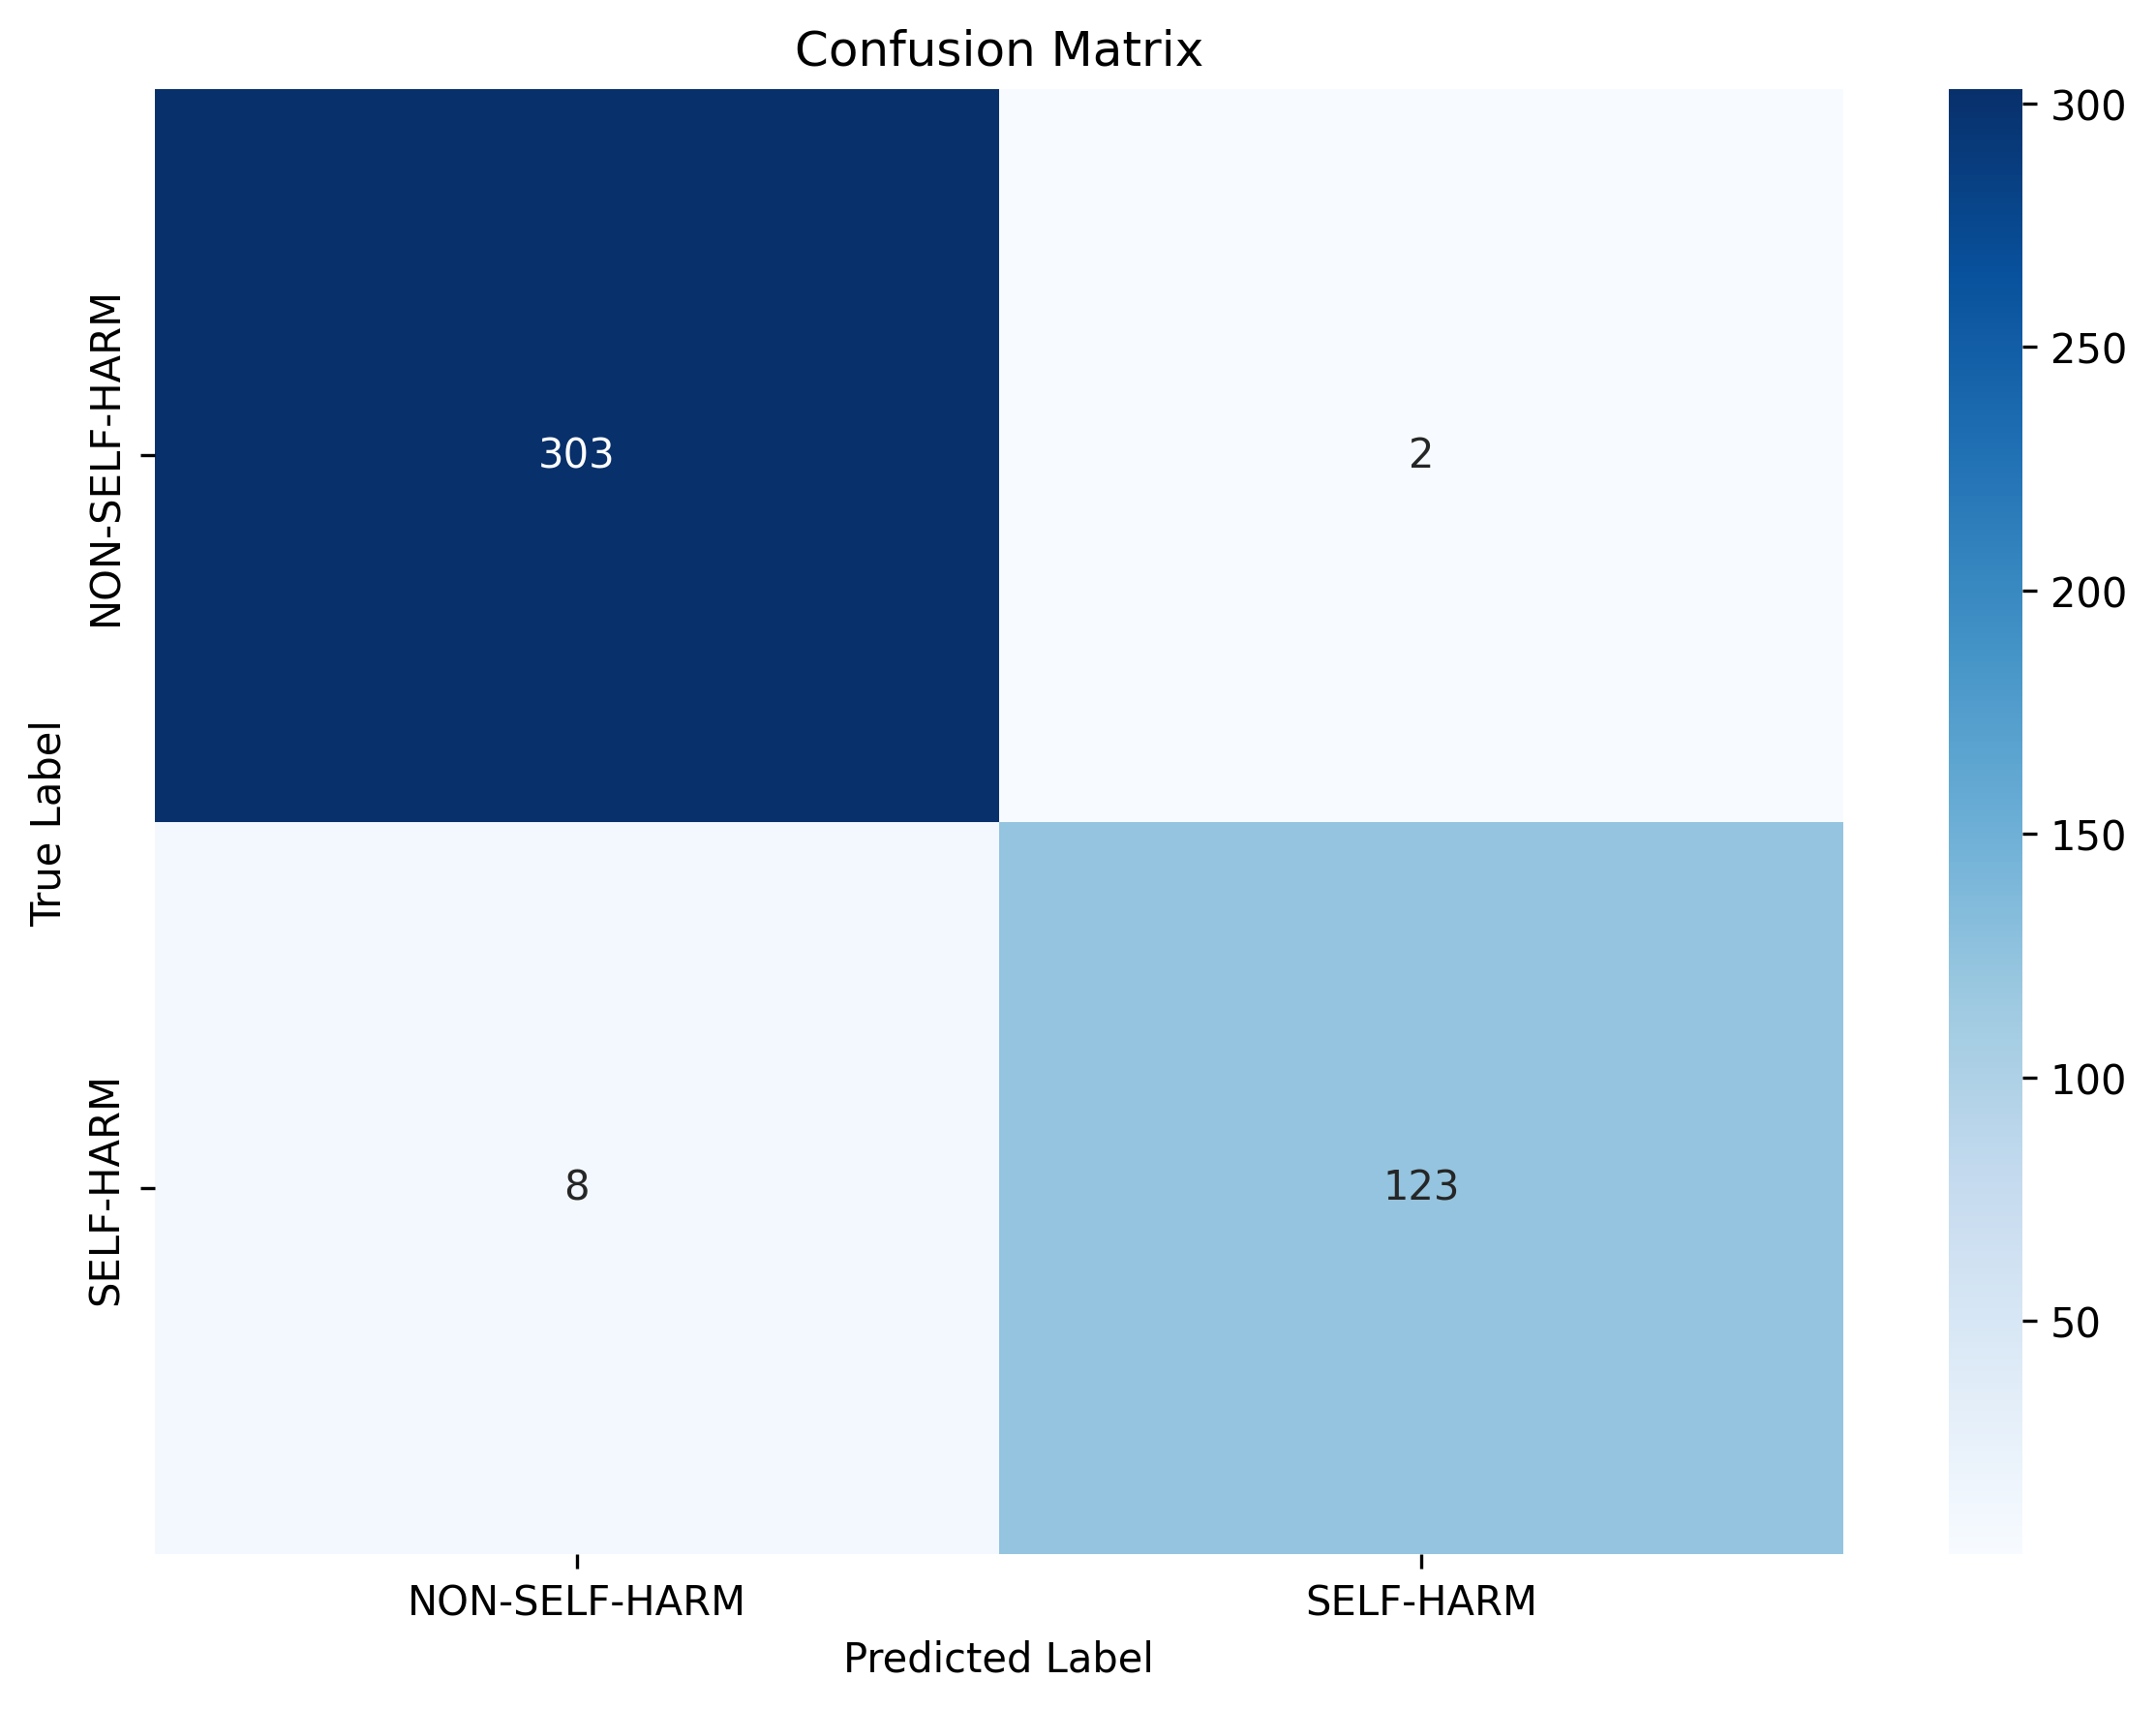
\includegraphics[width=0.5\textwidth]{figure/conf_E18.png}
\caption{\textit{Confusion Matrix} Eksperimen E18 pada Model Multimodal Gambar}
\label{fig:confusion_E18}
\end{figure}


Berdasarkan \textit{confusion matrix} pada eksperimen E18 yang dapat dilihat pada Gambar \ref{fig:confusion_E18} dengan strategi \textit{Focal Loss} ($\gamma = 2{,}0$), terlihat bahwa model menunjukkan performa yang sangat baik dan konsisten dengan metrik evaluasi yang diperoleh, yaitu \textit{accuracy} sebesar 97,7\%, \textit{precision} 98,4\%, \textit{recall} 93,9\%, dan \textit{F1-score} 96,1\%. Nilai \textit{precision} yang tinggi tercermin dari jumlah \textit{false positive} yang sangat kecil, yaitu hanya 2 data \textit{non-self-harm} yang salah diklasifikasikan sebagai \textit{self-harm}, sehingga model sangat akurat dalam memprediksi kelas positif. Sementara itu, nilai \textit{recall} yang tinggi namun belum sempurna disebabkan oleh masih adanya 8 data \textit{self-harm} yang tidak terdeteksi (\textit{false negative}), yang menunjukkan bahwa meskipun \textit{Focal Loss} mampu meningkatkan fokus pada sampel sulit, masih terdapat beberapa kasus yang sulit dikenali. Jumlah \textit{true positive} yang tinggi sebanyak 123 data menunjukkan bahwa sebagian besar konten \textit{self-harm} berhasil terdeteksi dengan baik. Kombinasi \textit{precision} dan \textit{recall} tersebut menghasilkan \textit{F1-score} yang tinggi, yang mengindikasikan keseimbangan performa klasifikasi yang optimal. Secara keseluruhan, hasil ini menunjukkan bahwa penggunaan \textit{Focal Loss} efektif dalam menangani ketidakseimbangan kelas dengan tetap menjaga akurasi dan sensitivitas model terhadap kelas minoritas.


\subsubsection{Pengaruh Metode \textit{Fusion}} \label{IV.MultimodalFusion}
Pada tahap ini, eksperimen dilakukan untuk menganalisis pengaruh metode \textit{fusion} dalam menggabungkan fitur gambar dan teks pada model multimodal. Eksperimen ini menggunakan varian model multimodal dengan pendekatan \textit{simple fusion}, di mana representasi fitur dari kedua modalitas digabungkan sebelum diteruskan ke \textit{MLP classifier}. Untuk menjaga konsistensi evaluasi, konfigurasi \textit{hyperparameter} pelatihan yang digunakan sama seperti pada Tabel \ref{table:4.distribusi_label}, dengan menggunakan dimensi terbaik hasil eksperimen sebelumnya, yaitu 256 untuk teks dan 256 untuk gambar. Selain itu, strategi \textit{loss} yang digunakan pada seluruh eksperimen ini adalah \textit{Focal Loss}, yang telah terbukti memberikan performa terbaik dalam menangani ketidakseimbangan kelas pada tahap sebelumnya.

Berdasarkan hasil eksperimen metode \textit{fusion}, terlihat bahwa seluruh metode yang digunakan mampu menghasilkan performa yang relatif tinggi dan stabil, dengan nilai \textit{accuracy} dan \textit{F1-score} yang berada pada kisaran yang tidak jauh berbeda. Metode \textit{concatenate} pada eksperimen E20 menunjukkan performa terbaik dengan \textit{accuracy} sebesar 97,7\% dan \textit{F1-score} sebesar 96,1\%, yang sebanding dengan beberapa metode \textit{fusion} lainnya seperti \textit{gated fusion} dan \textit{Attention Fusion}. Hal ini menunjukkan bahwa penggabungan fitur secara sederhana melalui \textit{concatenation} sudah cukup efektif dalam merepresentasikan informasi dari kedua modalitas tanpa memerlukan mekanisme yang lebih kompleks. Sebaliknya, metode seperti \textit{addition} dan \textit{multiplication} menunjukkan performa yang sedikit lebih rendah, yang mengindikasikan bahwa pendekatan \textit{element-wise} kurang mampu menangkap interaksi antar modalitas secara optimal.


\begin{table}[H]
    \centering
    \caption{Hasil Eksperimen Model Multimodal Metode \textit{Fusion}}
    \label{table:4.multimodal_fusion}
    \scriptsize
    \setlength{\tabcolsep}{2pt}
    \renewcommand{\arraystretch}{1.1}
    \resizebox{\textwidth}{!}{%
        \begin{tabular}{llcccccccccc}
            \hline
            \textbf{Kode} & \textbf{Metode \textit{Fusion}} & \textbf{\textit{Acc} (\%)} & \textbf{\textit{Prec} (\%)} & \textbf{\textit{Rec} (\%)} & \textbf{\textit{F1} (\%)} & \textbf{TP} & \textbf{TN} & \textbf{FP} & \textbf{FN} & \shortstack{\textbf{Best}\\\textbf{Epc}} & \shortstack{\textbf{Val}\\\textbf{Loss}} \\
            \hline
            \textbf{E20} & \textbf{\textit{Concatenate}} & \textbf{97,7} & \textbf{98,4} & \textbf{93,9} & \textbf{96,1} & \textbf{123} & \textbf{303} & \textbf{2} & \textbf{8} & \textbf{9} & \textbf{0,03} \\
            E21 & \textit{Addition} (\textit{Sum}) & 97,5 & 98,4 & 93,1 & 95,7 & 122 & 303 & 2 & 9 & 7 & 0,03 \\
            E22 & \textit{Multiplication} & 97,5 & 97,6 & 93,9 & 95,7 & 123 & 302 & 3 & 8 & 7 & 0,03 \\
            E23 & \textit{Gated Fusion} & 97,7 & 99,2 & 93,1 & 96,1 & 122 & 304 & 1 & 9 & 4 & 0,03 \\
            E24 & \textit{Attention Fusion} & 97,7 & 98,4 & 93,9 & 96,1 & 123 & 303 & 2 & 8 & 6 & 0,03 \\
            E25 & \textit{Bilinear Fusion} & 97,5 & 96,9 & 94,7 & 95,8 & 124 & 301 & 4 & 7 & 7 & 0,04 \\
            \hline
        \end{tabular}
    }
    \smallskip
    \begin{flushleft}
    \footnotesize \textit{Catatan: Baris yang diformat tebal menunjukkan eksperimen dengan performa model terbaik.}
    \end{flushleft}
\end{table}


Meskipun metode \textit{fusion} yang lebih kompleks seperti \textit{gated fusion} dan \textit{attention fusion} menawarkan pendekatan yang lebih adaptif dalam memodelkan interaksi antar modalitas, hasil eksperimen menunjukkan bahwa peningkatan performa yang diperoleh tidak signifikan dibandingkan metode \textit{concatenate}. Oleh karena itu, metode \textit{concatenate} pada eksperimen E20 dipilih sebagai konfigurasi terbaik karena mampu menghasilkan performa yang tinggi dengan kompleksitas model yang lebih sederhana. Hal ini menunjukkan bahwa dalam penelitian ini, pendekatan sederhana sudah cukup efektif untuk menangkap hubungan antara fitur teks dan gambar, sehingga tidak diperlukan penambahan kompleksitas model yang lebih tinggi.Hal ini menunjukkan bahwa kompleksitas metode fusion tidak selalu berbanding lurus dengan peningkatan performa model. Pembahasan mengenai kurva pelatihan dan \textit{confusion matrix} pada konfigurasi terbaik ini mengacu pada hasil eksperimen sebelumnya dengan konfigurasi \textit{hyperparameter} dan strategi \textit{loss} yang sama.

\subsubsection{Model Multimodal Berbasis Transformer} \label{IV.MultimodalTransformer}
Pada tahap ini, dilakukan pengembangan arsitektur model multimodal dengan menambahkan \textit{Transformer Encoder} sebagai mekanisme untuk meningkatkan interaksi antar modalitas. Berbeda dengan pendekatan sebelumnya yang menggunakan \textit{simple fusion}, pada varian ini ditambahkan dua layer \textit{Transformer Encoder} setelah proses penggabungan fitur teks dan gambar untuk memodelkan hubungan lintas-modalitas secara lebih mendalam. Konfigurasi \textit{hyperparameter} yang digunakan tetap sama dengan eksperimen sebelumnya guna menjaga konsistensi evaluasi, termasuk penggunaan dimensi fitur terbaik yaitu 256 untuk teks dan 256 untuk gambar serta strategi \textit{loss} \textit{Focal Loss}. 

\begin{table}[H]
    \centering
    \caption{Hasil Eksperimen Model \textit{Multimodal Positional Embedding}}
    \label{table:4.multimodal_positional}
    \scriptsize
    \setlength{\tabcolsep}{2pt}
    \renewcommand{\arraystretch}{1.1}
    \resizebox{\textwidth}{!}{%
        \begin{tabular}{llcccccccccc}
            \hline
            \textbf{Kode} & \textbf{\textit{Positional Emb}} & \textbf{\textit{Acc} (\%)} & \textbf{\textit{Prec} (\%)} & \textbf{\textit{Rec} (\%)} & \textbf{\textit{F1} (\%)} & \textbf{TP} & \textbf{TN} & \textbf{FP} & \textbf{FN} & \shortstack{\textbf{Best}\\\textbf{Epc}} & \shortstack{\textbf{Val}\\\textbf{Loss}} \\
            \hline
            E26 & [Image, Text] & 97,5 & 98,4 & 93,1 & 95,7 & 122 & 303 & 2 & 9 & 8 & 0,09 \\
            E27 & [Text, Image] & 97,5 & 97,6 & 93,9 & 95,7 & 123 & 302 & 3 & 8 & 5 & 0,10 \\
            \hline
        \end{tabular}
    }
\end{table}


Berdasarkan hasil eksperimen variasi \textit{positional embedding} pada model multimodal berbasis \textit{Transformer} yang dapat dilihat pada Gambar \ref{fig:training_E26}, terlihat bahwa perubahan urutan token, baik [\textit{Image}, \textit{Text}] pada eksperimen E26 maupun [\textit{Text}, \textit{Image}] pada eksperimen E27, tidak memberikan perbedaan performa yang signifikan. Kedua konfigurasi menunjukkan nilai \textit{accuracy} dan \textit{F1-score} yang relatif sama, yaitu sebesar 97,5\% dan 95,7\%, dengan perbedaan kecil pada nilai \textit{precision} dan \textit{recall}. Hal ini menunjukkan bahwa model mampu mempelajari representasi multimodal secara efektif tanpa terlalu bergantung pada urutan token yang digunakan. Dengan demikian, pengaruh \textit{positional embedding} dalam eksperimen ini tidak terlalu dominan terhadap performa model, sehingga model cenderung \textit{robust} terhadap variasi urutan fitur yang diberikan.

\begin{figure}[H]
\centering
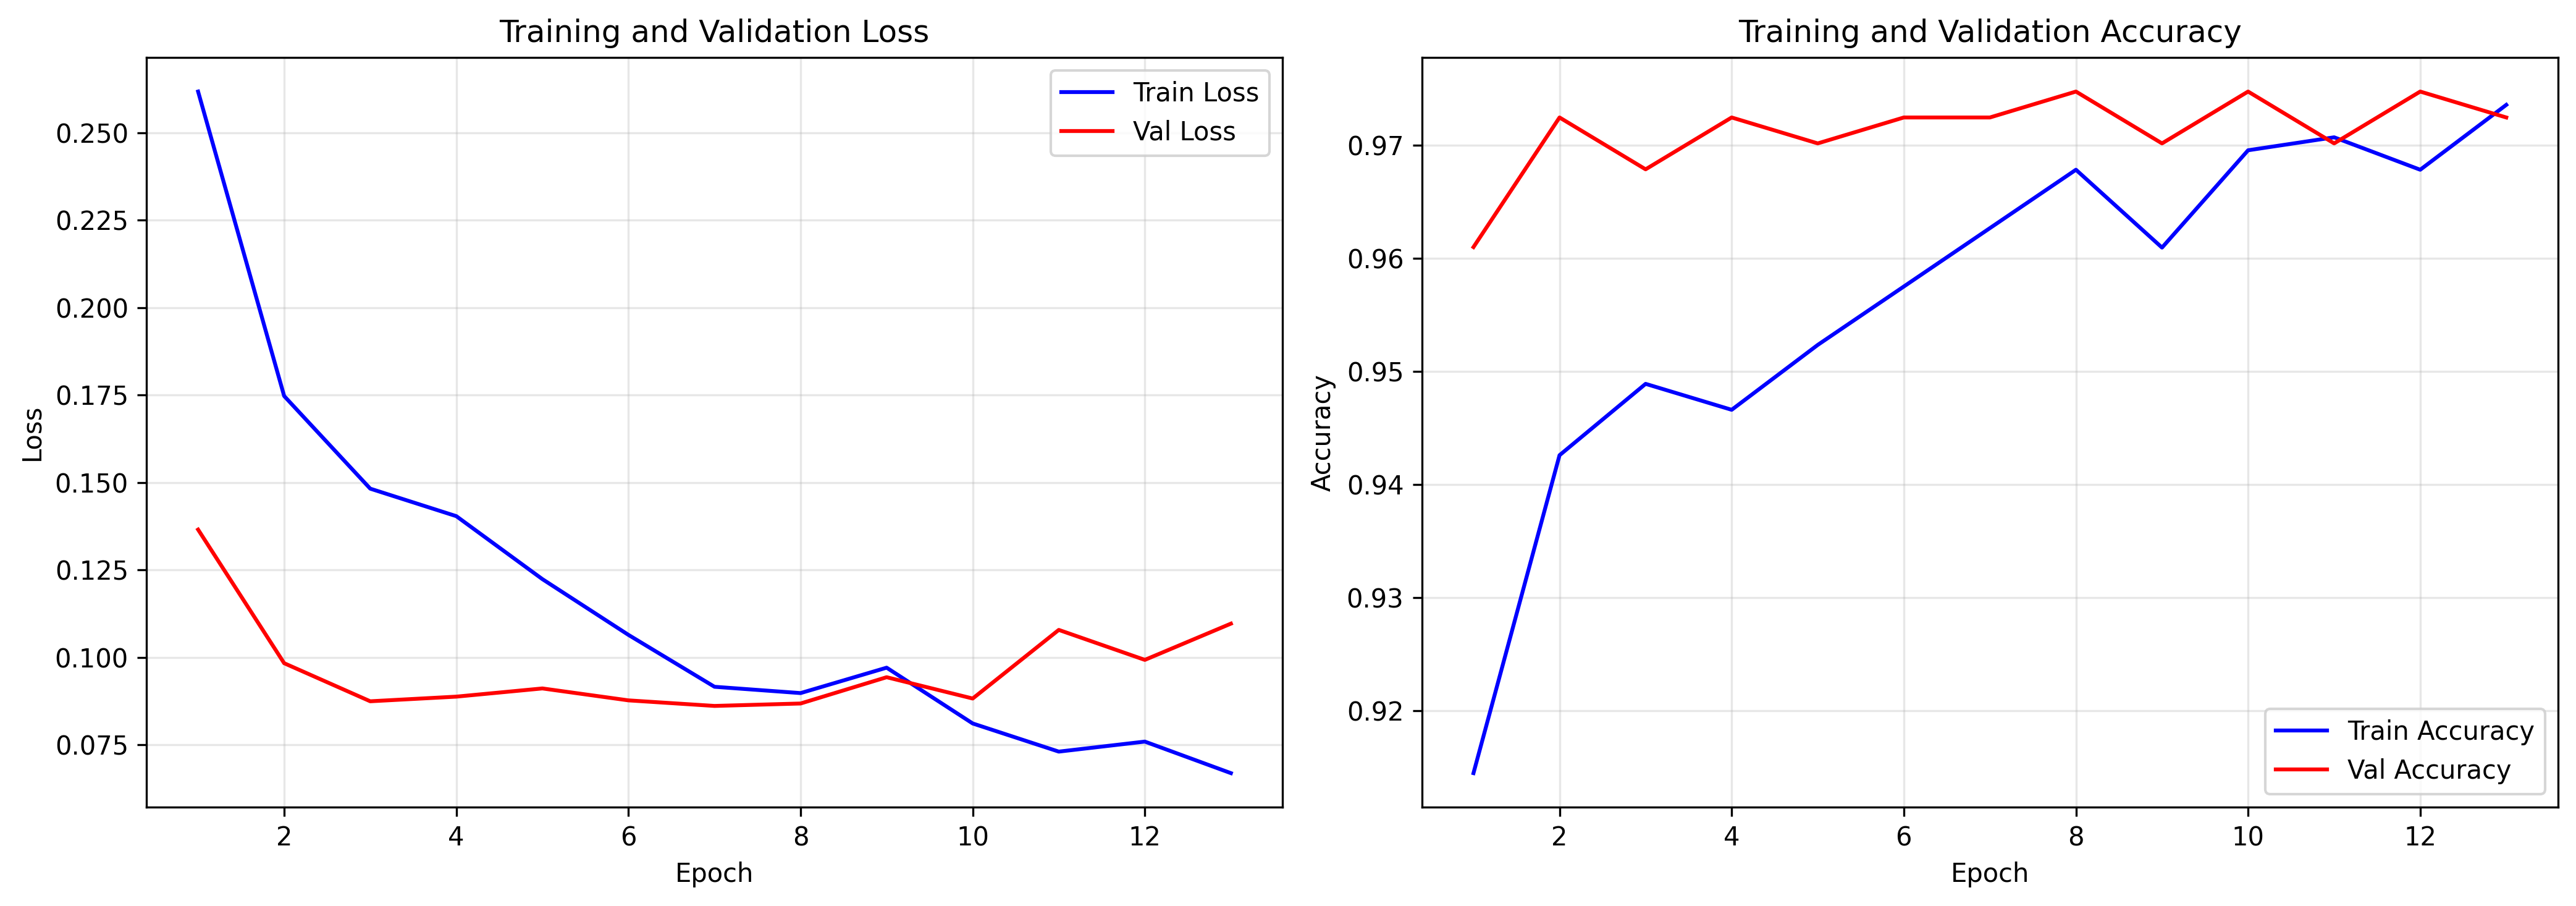
\includegraphics[width=1\textwidth]{figure/training_E26.png}
\caption{Kurva Pelatihan Eksperimen E26 pada Model Multimodal \textit{Positional Embedding}}
\label{fig:training_E26}
\end{figure}


Berdasarkan \textit{confusion matrix} pada eksperimen \textit{E26} dengan urutan \textit{positional embedding} [\textit{Image}, \textit{Text}], terlihat bahwa model memiliki performa yang sangat baik dan konsisten dengan metrik evaluasi yang diperoleh, yaitu \textit{accuracy} sebesar 97,5\%, \textit{precision} 98,4\%, \textit{recall} 93,1\%, dan \textit{F1-score} 95,7\%. Nilai \textit{precision} yang tinggi tercermin dari jumlah \textit{false positive} yang sangat kecil, yaitu hanya 2 data \textit{non-self-harm} yang salah diklasifikasikan sebagai \textit{self-harm}, sehingga model sangat akurat dalam memprediksi kelas positif. Sementara itu, nilai \textit{recall} yang sedikit lebih rendah disebabkan oleh masih adanya 9 data \textit{self-harm} yang tidak terdeteksi (\textit{false negative}), yang menunjukkan bahwa masih terdapat beberapa kasus yang sulit dikenali oleh model. Jumlah \textit{true positive} yang tinggi sebanyak 122 data menunjukkan bahwa sebagian besar konten \textit{self-harm} berhasil terdeteksi dengan baik. Secara keseluruhan, kombinasi \textit{precision} dan \textit{recall} tersebut menghasilkan \textit{F1-score} yang tinggi, yang mengindikasikan keseimbangan performa klasifikasi yang optimal pada model multimodal berbasis \textit{Transformer}.

\begin{figure}[H]
\centering
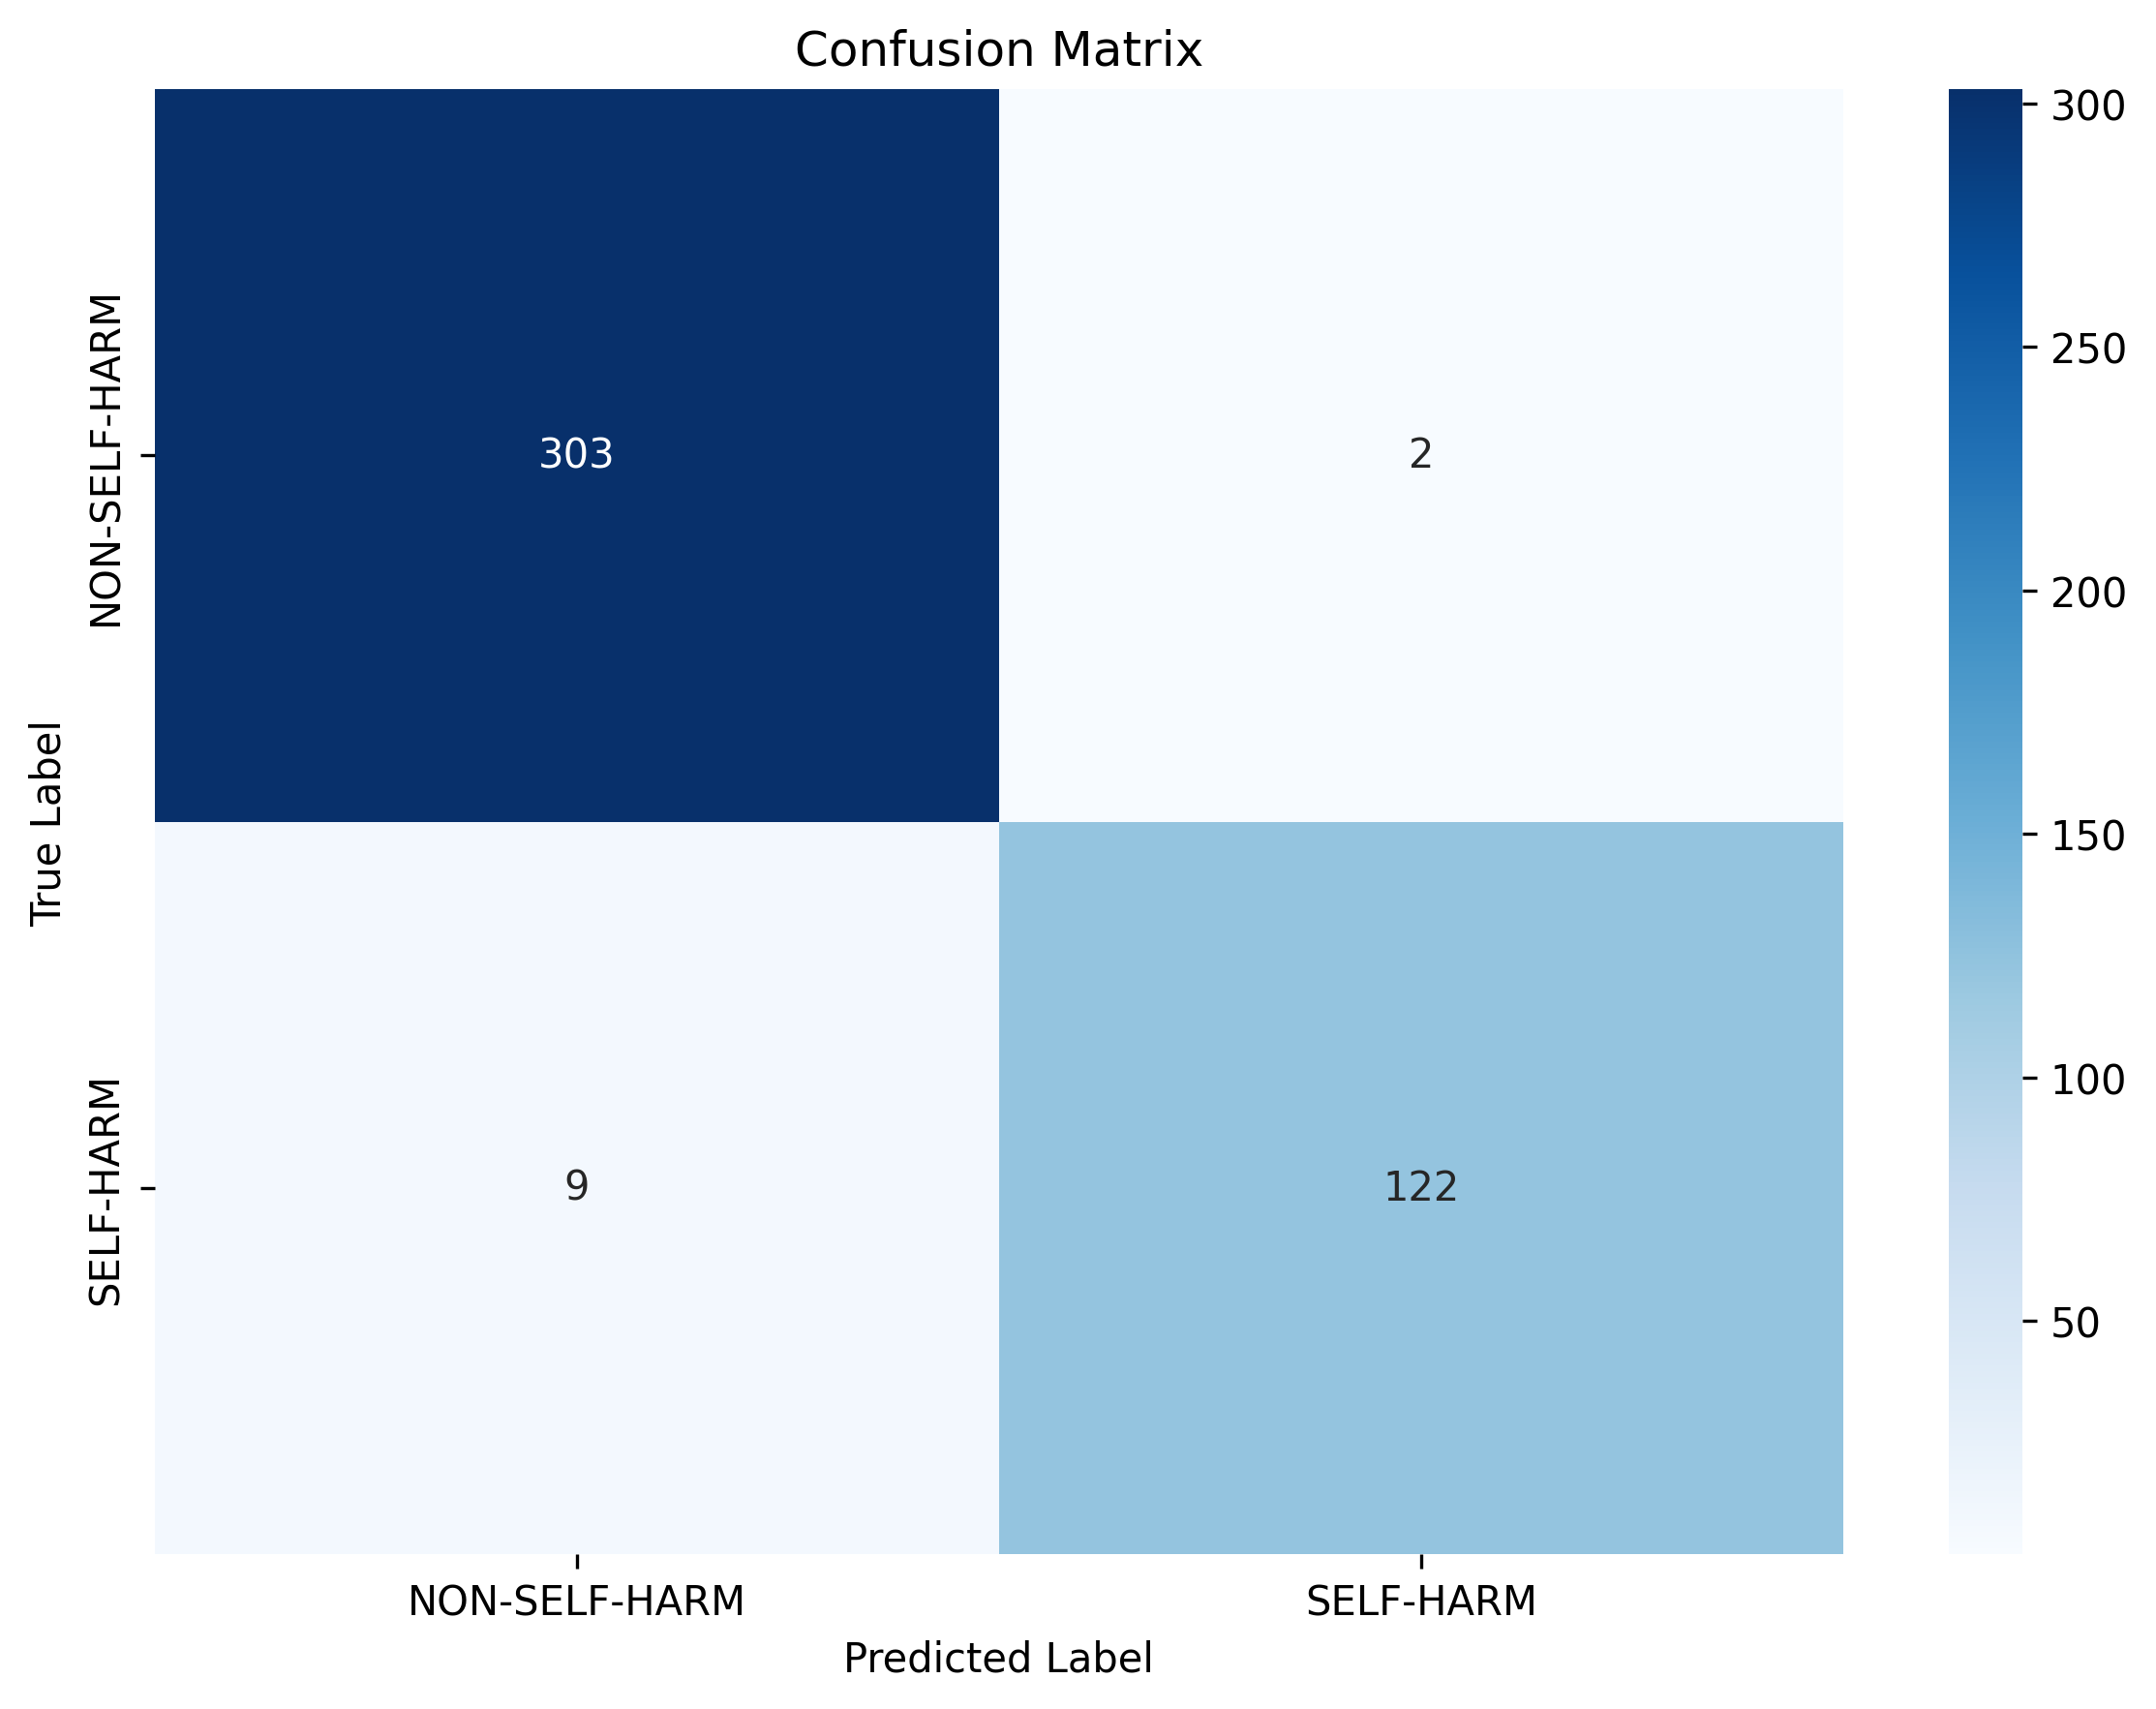
\includegraphics[width=0.7\textwidth]{figure/conf_E26.png}
\caption{\textit{Confusion Matrix} Eksperimen E26 pada Model \textit{Multimodal Positional Embedding}}
\label{fig:confusion_E26}
\end{figure}

Jika dibandingkan dengan model multimodal berbasis \textit{simple fusion} pada eksperimen sebelumnya, penggunaan \textit{Transformer Encoder} tidak menunjukkan peningkatan performa yang signifikan. Model terbaik pada pendekatan \textit{simple fusion}, yaitu eksperimen E18 dengan \textit{Focal Loss}, menghasilkan \textit{F1-score} sebesar 96,1\%, sedangkan model berbasis \textit{Transformer} pada eksperimen E26 menghasilkan \textit{F1-score} sebesar 95,7\%. Perbedaan performa yang relatif kecil ini menunjukkan bahwa meskipun \textit{Transformer} mampu memodelkan interaksi antar modalitas secara lebih kompleks, peningkatan tersebut tidak memberikan keuntungan yang berarti dibandingkan pendekatan yang lebih sederhana. Dengan demikian, dalam penelitian ini, peningkatan kompleksitas arsitektur tidak selalu berbanding lurus dengan peningkatan performa model. Hal ini menunjukkan bahwa pendekatan \textit{simple fusion} sudah cukup efektif dalam menangkap hubungan antara fitur teks dan gambar, sehingga tidak diperlukan penambahan kompleksitas model yang lebih tinggi melalui penggunaan \textit{Transformer Encoder}.


\subsection{Perbandingan dan Analisis Model} \label{IV.Perbandingan}
Pada tahap ini dilakukan analisis perbandingan performa antara model unimodal dan model multimodal untuk mengevaluasi efektivitas pendekatan yang diusulkan dalam penelitian ini. Perbandingan dilakukan dengan menggunakan metrik evaluasi utama, yaitu \textit{accuracy}, \textit{precision}, \textit{recall}, dan \textit{F1-score}, untuk melihat perbedaan kinerja masing-masing model dalam mendeteksi konten \textit{self-harm}. Model unimodal yang hanya memanfaatkan satu jenis modalitas dibandingkan dengan model multimodal yang mengintegrasikan representasi visual dan tekstual melalui pendekatan \textit{intermediate fusion}. Analisis ini bertujuan untuk mengidentifikasi sejauh mana integrasi kedua modalitas mampu meningkatkan pemahaman konteks dalam meme serta memberikan performa klasifikasi yang lebih optimal.

\begin{table}[H]
    \centering
    \caption{Perbandingan Performa Model}
    \label{table:4.perbandingan_model}
    \small
    \setlength{\tabcolsep}{6pt} % Jarak kolom lebih lega karena jumlah kolom sedikit
    \renewcommand{\arraystretch}{1.2}
    
    \resizebox{\textwidth}{!}{%
        \begin{tabular}{llcccc}
            \hline
            \textbf{Model} & \textbf{Kode} & \textbf{\textit{Acc}} & \textbf{\textit{Prec}} & \textbf{\textit{Rec}} & \textbf{\textit{F1}} \\
            \hline
            \textit{Unimodal Image} & E4 & 95,2\% & 97,4\% & 86,3\% & 91,5\% \\
            \textit{Unimodal Text} & E6 & 95,4\% & 96,6\% & 87,8\% & 92,0\% \\
            \textbf{Multimodal Simple} & \textbf{E18} & \textbf{97,7\%} & \textbf{98,4\%} & \textbf{93,9\%} & \textbf{96,1\%} \\
            \textit{Multimodal Transformer} & E26 & 97,5\% & 98,4\% & 93,1\% & 95,7\% \\
            \hline
        \end{tabular}
    }
    \smallskip
    \begin{flushleft}
    \small \textit{Catatan: Baris yang diformat tebal menunjukkan performa model terbaik.}
    \end{flushleft}
\end{table}

Berdasarkan Tabel \ref{table:4.perbandingan_model}, terlihat bahwa model multimodal secara konsisten memberikan performa yang lebih baik dibandingkan model unimodal, baik pada metrik \textit{accuracy}, \textit{precision}, \textit{recall}, maupun \textit{F1-score}. Model unimodal gambar E4 dan unimodal teks E6 masing-masing hanya mampu mencapai \textit{F1-score} sebesar 91,5\% dan 92,0\%, yang menunjukkan keterbatasan dalam menangkap konteks meme secara menyeluruh ketika hanya mengandalkan satu modalitas. Sebaliknya, model multimodal \textit{simple fusion} E18 mampu meningkatkan performa secara signifikan dengan \textit{F1-score} sebesar 96,1\% dan \textit{recall} sebesar 93,9\%. Peningkatan ini menunjukkan bahwa integrasi representasi visual dan tekstual melalui pendekatan multimodal mampu memberikan pemahaman konteks yang lebih lengkap, sehingga model lebih efektif dalam mendeteksi konten \textit{self-harm}.

Jika dibandingkan antara dua pendekatan multimodal, yaitu \textit{simple fusion} dan \textit{Transformer}, terlihat bahwa penggunaan \textit{Transformer Encoder} tidak memberikan peningkatan performa yang signifikan. Model multimodal berbasis \textit{Transformer} E26 menghasilkan \textit{F1-score} sebesar 95,7\%, yang sedikit lebih rendah dibandingkan model \textit{simple fusion}. Hal ini menunjukkan bahwa meskipun \textit{Transformer} memiliki kemampuan untuk memodelkan interaksi antar modalitas secara lebih kompleks, pendekatan tersebut tidak memberikan pengaruh yang signifikan dalam penelitian ini. Dengan demikian, dapat disimpulkan bahwa metode \textit{simple fusion} sudah cukup efektif dalam menggabungkan fitur teks dan gambar, sehingga tidak diperlukan peningkatan kompleksitas arsitektur untuk mencapai performa yang optimal.

Berdasarkan seluruh hasil eksperimen yang telah dilakukan,  model multimodal yang dibangun dengan mengintegrasikan CLIP sebagai \textit{encoder} visual dan ELECTRA sebagai \textit{encoder} tekstual melalui pendekatan \textit{intermediate fusion} mampu memberikan performa yang lebih baik dibandingkan model unimodal. Hal ini ditunjukkan oleh peningkatan nilai \textit{F1-score} dari 91,5\% pada model unimodal gambar dan 92,0\% pada model unimodal teks menjadi 96,1\% pada model multimodal. Selain itu, evaluasi menggunakan \textit{confusion matrix} menunjukkan bahwa model multimodal memiliki kemampuan yang lebih baik dalam mendeteksi kelas \textit{self-harm}, khususnya dalam meningkatkan nilai \textit{recall} dan mengurangi kesalahan klasifikasi.

\subsection{Evaluasi oleh \textit{Annotator} Manusia} \label{IV.EvaluasiAnnotator}
Pada tahap ini digunakan sebanyak 19 data meme yang dianotasi oleh dua \textit{annotator} independen dengan latar belakang yang berbeda, di mana masing-masing \textit{annotator} memberikan label serta tingkat keyakinan (\textit{confidence}) terhadap setiap data. Berdasarkan hasil anotasi yang diperoleh, sebagian besar data menunjukkan kesesuaian label antar \textit{annotator} (\textit{agreement}), sementara sebagian lainnya mengalami perbedaan interpretasi (\textit{disagreement}). Distribusi tingkat kesepakatan antar \textit{annotator} dapat dilihat pada Tabel \ref{tab:agreement_disagreement} di bawah ini.

\begin{table}[H]
    \centering
    \caption{Distribusi \textit{Agreement} dan \textit{Disagreement} Annotator}
    \label{tab:agreement_disagreement}
    \small
    \setlength{\tabcolsep}{4pt}
    \renewcommand{\arraystretch}{1.2}
    \begin{tabular}{>{\centering\arraybackslash}m{3cm} >{\centering\arraybackslash}m{2.8cm}}
        \hline
        \textbf{Kategori} & \textbf{Jumlah Data} \\
        \hline
        \textit{Agreement} & 14 \\
        \textit{Disagreement} & 5 \\
        \hline
        \textbf{Total} & \textbf{19} \\
        \hline
    \end{tabular}
\end{table}

Berdasarkan Tabel \ref{tab:agreement_disagreement}, terlihat bahwa sebanyak 14 data memiliki kesesuaian label antar \textit{annotator}, yang menunjukkan bahwa sebagian besar meme masih dapat diinterpretasikan secara relatif konsisten. Namun, terdapat 5 data yang mengalami \textit{disagreement}, yang mengindikasikan adanya tingkat ambiguitas dalam interpretasi, khususnya pada meme dengan makna implisit dan konteks yang kompleks. Untuk menangani  ketidaksepakatan label oleh dua \textit{annotator}, dilakukan proses peninjauan ulang secara manual oleh peneliti  dengan mengacu pada \textit{annotation guideline} yang telah ditetapkan. Proses ini bertujuan untuk menentukan label akhir (\textit{ground truth}) yang konsisten, sehingga tidak bergantung pada satu perspektif \textit{annotator} saja. Selain itu, tingkat keyakinan (\textit{confidence}) yang diberikan oleh \textit{annotator} digunakan sebagai informasi tambahan untuk memahami tingkat kesulitan interpretasi pada setiap data, meskipun tidak digunakan sebagai dasar utama dalam penentuan label akhir.

\begin{figure}[H]
\centering

\includegraphics[width=0.37\textwidth]{figure/datatest.png}
\caption{Contoh Data dengan \textit{Disagreement} Antar \textit{Annotator}}
\label{fig:datatest}
\end{figure}

Salah satu contoh kasus \textit{disagreement} ditunjukkan pada Gambar \ref{fig:datatest}. meme tersebut menampilkan teks ``\textit{you should krill yourself NOW}'' yang dipadukan dengan gambar menyerupai \textit{krill} (udang kecil) dalam suasana dramatis. \textit{Annotator} pertama memberikan label \textit{self-harm} dengan tingkat keyakinan 0,8, sedangkan \textit{annotator} kedua memberikan label \textit{non self-harm} dengan tingkat keyakinan yang sama, yaitu 0,8. Perbedaan interpretasi ini disebabkan oleh adanya permainan kata (\textit{wordplay}) pada kata ``\textit{krill}'', yang secara fonetik menyerupai kata ``\textit{kill}'' yang memiliki konotasi ajakan untuk melukai diri sendiri. Dari sisi visual, penggunaan gambar \textit{krill} dapat dipahami sebagai elemen humor yang tidak secara langsung menunjukkan indikasi berbahaya.

Namun, jika dilihat dari kombinasi teks dan makna implisitnya, frasa tersebut dapat diinterpretasikan sebagai bentuk penyamaran dari ungkapan ``\textit{kill yourself}'', yang merupakan indikator kuat dari konten \textit{self-harm}. Berdasarkan peninjauan ulang oleh peneliti dengan mengacu pada \textit{annotation guideline}, label akhir pada kasus tersebut ditetapkan sebagai \textit{self-harm}. Keputusan ini diambil dengan mempertimbangkan bahwa makna implisit dari teks memiliki indikasi yang lebih kuat dibandingkan interpretasi literal dari visual, sehingga keseluruhan konteks multimodal tetap mengarah pada konten yang berpotensi berbahaya. Perbedaan interpretasi antar \textit{annotator} umumnya terjadi pada meme yang mengandung unsur ambiguitas, seperti penggunaan humor gelap, sarkasme, serta permainan kata (\textit{wordplay}) yang dapat menghasilkan lebih dari satu makna. Berikut distribusi label akhir  yang dikategorikan sebagai \textit{self-harm} dan \textit{non self-harm} setelah dilakukan peninjauan ulang secara manual oleh peneliti.

\begin{table}[H]
    \centering
    \caption{Distribusi Label \textit{Ground Truth} Annotator}
    \label{tab:ground_truth_annotator}
    \small
    \setlength{\tabcolsep}{6pt}
    \renewcommand{\arraystretch}{1.2}
    \begin{tabular}{p{3cm} p{2cm}}
        \hline
        \textbf{Label} & \textbf{Jumlah Data} \\
        \hline
        \textit{Self-harm} & 14 \\
        \textit{Non self-harm} & 5 \\
        \hline
        \textbf{Total} & \textbf{19} \\
        \hline
    \end{tabular}
\end{table}

Selanjutnya, dilakukan evaluasi terhadap hasil prediksi model dengan membandingkannya terhadap label \textit{ground truth} yang telah ditentukan berdasarkan anotasi manusia. Berdasarkan hasil pengujian terhadap 19 data uji, diperoleh distribusi hasil prediksi yang kemudian dirangkum dalam \textit{confusion matrix} pada Tabel \ref{tab:confusion_matrix_ground_truth}.

\begin{table}[H]
    \centering
    \caption{\textit{Confusion Matrix} Model terhadap \textit{Ground Truth}}
    \label{tab:confusion_matrix_ground_truth}
    \small
    \setlength{\tabcolsep}{6pt}
    \renewcommand{\arraystretch}{1.2}
    \begin{tabular}{p{3cm} >{\centering\arraybackslash}m{2.2cm} >{\centering\arraybackslash}m{2.6cm}}
        \hline
        & \textit{Pred: Self-harm} & \textit{Pred: Non self-harm} \\
        \hline
        \textit{Actual Self-harm} & 8 & 6 \\
        \textit{Actual Non self-harm} & 1 & 4 \\
        \hline
    \end{tabular}
\end{table}

Berdasarkan \textit{confusion matrix} tersebut, diperoleh nilai \textit{accuracy} sebesar 63,2\%, yang menunjukkan bahwa model mampu mengklasifikasikan sebagian data dengan benar. Nilai \textit{precision} sebesar 88,9\% menunjukkan bahwa sebagian besar prediksi \textit{self-harm} yang dihasilkan oleh model merupakan prediksi yang tepat. Namun, nilai \textit{recall} yang relatif rendah, yaitu sebesar 57,1\%, menunjukkan bahwa model masih belum mampu mendeteksi seluruh konten \textit{self-harm}, khususnya pada data yang bersifat ambigu. Nilai \textit{F1-score} sebesar 69,6\% menunjukkan keseimbangan antara \textit{precision} dan \textit{recall} dalam performa model. Meskipun model memiliki tingkat ketepatan yang cukup tinggi dalam mendeteksi \textit{self-harm}, masih terdapat sejumlah kasus \textit{false negative}, yaitu ketika konten \textit{self-harm} tidak berhasil terdeteksi oleh model dan justru diklasifikasikan sebagai \textit{non self-harm}.

\begin{figure}[H]
    \centering
    \begin{minipage}[b]{0.4\textwidth}
        \centering
        
\includegraphics[width=\linewidth]{figure/fp1.png}
    \end{minipage}
    \hfill
    \begin{minipage}[b]{0.4\textwidth}
        \centering
        
\includegraphics[width=\linewidth]{figure/fp2.png}
    \end{minipage}
    \caption{Contoh \textit{False Negative} pada Model}
    \label{fig:false_negative_examples}
\end{figure}

Gambar di atas menunjukkan dua contoh meme yang termasuk dalam kategori \textit{false negative}, yaitu model gagal mendeteksi konten \textit{self-harm} dan mengklasifikasikannya sebagai \textit{non self-harm}. Pada kedua kasus tersebut, label \textit{ground truth} berdasarkan anotasi manusia adalah \textit{self-harm}, namun model memberikan prediksi yang berbeda. Pada gambar pertama, meme menampilkan teks ``\textit{I'm here to post memes and kill myself... and I'm all out of memes}'' yang mengandung unsur humor gelap dan sarkasme. Visual yang ditampilkan berupa karakter manusia dengan konteks yang tidak secara langsung menunjukkan tindakan \textit{self-harm}. Kedua \textit{annotator} mengklasifikasikan meme ini sebagai \textit{self-harm}. Namun, model gagal mendeteksi konteks tersebut dan mengklasifikasikannya sebagai \textit{non self-harm} dengan tingkat \textit{confidence} 0,62. Gambar kedua, meme menampilkan teks ``\textit{I'm going to kill myself}'' yang secara eksplisit mengandung indikasi \textit{self-harm}, dipadukan dengan karakter animasi yang bersifat humor. Kedua \textit{annotator} sepakat bahwa meme ini termasuk dalam kategori \textit{self-harm}. Namun, model mengklasifikasikan sebagai \textit{non self-harm}. Hal ini menunjukkan bahwa model kemungkinan terpengaruh oleh elemen visual yang tidak berbahaya, sehingga mengurangi sensitivitas terhadap teks yang memiliki makna eksplisit.



Kedua contoh tersebut menunjukkan bahwa model masih memiliki keterbatasan dalam memahami konteks multimodal secara menyeluruh, khususnya pada kasus di mana terdapat konflik antara teks dan visual. Model cenderung lebih terpengaruh oleh elemen visual yang bersifat netral atau humor, sehingga gagal menangkap makna teks yang mengandung indikasi \textit{self-harm}. Selain itu, penggunaan bahasa yang bersifat sarkastik atau tidak literal juga menjadi tantangan tersendiri bagi model, terutama jika pola tersebut tidak banyak muncul dalam data pelatihan.

\begin{figure}[H]
    \centering
    
\includegraphics[width=0.5\textwidth]{figure/fn1.png}
    \caption{Contoh \textit{False Positive} pada Model}
    \label{fig:false_positive_example}
\end{figure}

Gambar di atas menunjukkan contoh meme yang termasuk dalam kategori \textit{false positive}, yaitu model mengklasifikasikan sebagai \textit{self-harm}, berdasarkan \textit{ground truth} termasuk dalam kategori \textit{non self-harm}. Pada kasus ini, model memberikan prediksi \textit{self-harm} dengan nilai \textit{confidence} sebesar 0,52. Berdasarkan hasil anotasi, terdapat perbedaan interpretasi antara \textit{annotator}. \textit{Annotator} pertama mengklasifikasikan meme tersebut sebagai \textit{non self-harm}, sedangkan \textit{annotator} kedua memberikan label \textit{self-harm}. Perbedaan ini menunjukkan bahwa meme tersebut bersifat ambigu dan dapat ditafsirkan dari berbagai perspektif. Namun, setelah dilakukan proses peninjauan ulang oleh peneliti dengan mengacu pada \textit{annotation guideline}, label akhir ditetapkan sebagai \textit{non self-harm}.

Secara konteks, meme ini menampilkan teks ``\textit{me: i'm fine, my therapist:}'' yang mengarah pada ekspresi kondisi emosional atau tekanan psikologis, namun tidak secara eksplisit maupun implisit menunjukkan adanya indikasi tindakan \textit{self-harm}. Visual yang ditampilkan juga memperkuat ekspresi emosional tanpa adanya simbol atau konteks yang berkaitan langsung dengan perilaku melukai diri sendiri. Kesalahan klasifikasi oleh model pada kasus ini kemungkinan disebabkan oleh sensitivitas model terhadap kata-kata atau konteks emosional yang berkaitan dengan kondisi mental, sehingga cenderung mengasosiasikannya sebagai \textit{self-harm}. Hal ini menunjukkan bahwa model masih memiliki keterbatasan dalam membedakan antara ekspresi emosional umum dengan indikasi \textit{self-harm} yang sebenarnya. Contoh ini memperkuat temuan sebelumnya bahwa selain \textit{false negative}, model juga mengalami \textit{false positive} pada data yang bersifat ambigu. Hal ini menunjukkan bahwa tantangan utama dalam deteksi konten \textit{self-harm} tidak hanya terletak pada pemahaman makna implisit, tetapi juga pada kemampuan model dalam membedakan konteks emosional yang tidak berbahaya dengan indikasi konten berisiko.

\clearpage

